%%
%% Beginning of file 'hoffart-lamberti-459-final.tex'
%%
%% Modified 2017 March
%%
%% This is a manuscript marked up using the AASTeX v6.1 LaTeX 2e macros.
%%
%% AASTeX is now based on Alexey Vikhlinin's emulateapj.cls
%% (Copyright 2000-2015).  See the classfile for details.
%%
%% AASTeX requires revtex4-1.cls (http://publish.aps.org/revtex4/) and
%% other external packages (latexsym, graphicx, amssymb, longtable, and epsf).
%% All of these external packages should already be present in the modern TeX
%% distributions.  If not they can also be obtained at www.ctan.org.
%%
%%
%% Using aastex version 6.1

\documentclass[twocolumn]{aastex61}
\usepackage{amsmath}
\usepackage{mathtools}
\usepackage{amssymb}
\usepackage{graphicx}

% \usepackage{tabularx}

\usepackage[caption=false]{subfig}

%% The default is a single spaced, 10 point font article.
%% There are 5 other style options available via an optional argument. They
%% can be envoked like this:
%%
%% \documentclass[argument]{aastex61}
%%
%% where the arguement options are:
%%
%%  twocolumn   : two text columns, 10 point font, single spaced article.
%%                This is the most compact and represent the final published
%%                derived PDF copy of the accepted manuscript from the publisher
%%  manuscript  : one text column, 12 point font, double spaced article.
%%  preprint    : one text column, 12 point font, single spaced article.
%%  preprint2   : two text columns, 12 point font, single spaced article.
%%  modern      : a stylish, single text column, 12 point font, article with
%% 		  wider left and right margins. This uses the Daniel
%% 		  Foreman-Mackey and David Hogg design.
%%
%% Note that you can submit to the AAS Journals in any of these 6 styles.
%%
%% There are other optional arguments one can envoke to allow other stylistic
%% actions. The available options are:
%%
%%  astrosymb    : Loads Astrosymb font and define \astrocommands.
%%  tighten      : Makes baselineskip slightly smaller, only works with
%%                 the twocolumn substyle.
%%  times        : uses times font instead of the default
%%  linenumbers  : turn on lineno package.
%%  trackchanges : required to see the revision mark up and print its output
%%  longauthor   : Do not use the more compressed footnote style (default) for
%%                 the author/collaboration/affiliations. Instead print all
%%                 affiliation information after each name. Creates a much
%%                 long author list but may be desirable for short author papers
%%
%% these can be used in any combination, e.g.
%%
%% \documentclass[twocolumn,linenumbers,trackchanges]{aastex61}

%% AASTeX v6.* now includes \hyperref support. While we have built in specific
%% defaults into the classfile you can manually override them with the
%% \hypersetup command. For example,
%%
%%\hypersetup{linkcolor=red,citecolor=green,filecolor=cyan,urlcolor=magenta}
%%
%% will change the color of the internal links to red, the links to the
%% bibliography to green, the file links to cyan, and the external links to
%% magenta. Additional information on \hyperref options can be found here:
%% https://www.tug.org/applications/hyperref/manual.html#x1-40003

%% If you want to create your own macros, you can do so
%% using \newcommand. Your macros should appear before
%% the \begin{document} command.
%%
\newcommand{\vdag}{(v)^\dagger}
\newcommand\aastex{AAS\TeX}
\newcommand\latex{La\TeX}

%% Reintroduced the \received and \accepted commands from AASTeX v5.2

\received{\today}

%% \revised{}
%% \accepted{}
%% Command to document which AAS Journal the manuscript was submitted to.
%% Adds "Submitted to " the arguement.
  %\submitjournal{ApJ}

%% Mark up commands to limit the number of authors on the front page.
%% Note that in AASTeX v6.1 a \collaboration call (see below) counts as
%% an author in this case.
%%
%%\AuthorCollaborationLimit=3
%%
%% Note that all of the author will be shown in the published article.
%% This feature is meant to be used prior to acceptance to make the
%% front end of a long author article more manageable. Please do not use
%% this functionality for manuscripts with less than 20 authors. Conversely,
%% please do use this when the number of authors exceeds 40.
%%
%% Use \allauthors at the manuscript end to show the full author list.
%% This command should only be used with \AuthorCollaborationLimit is used.

%% The following command can be used to set the latex table counters.  It
%% is needed in this document because it uses a mix of latex tabular and
%% AASTeX deluxetables.  In general it should not be needed.
%\setcounter{table}{1}

%%%%%%%%%%%%%%%%%%%%%%%%%%%%%%%%%%%%%%%%%%%%%%%%%%%%%%%%%%%%%%%%%%%%%%%%%%%%%%%%
%%
%% The following section outlines numerous optional output that
%% can be displayed in the front matter or as running meta-data.
%%
%% If you wish, you may supply running head information, although
%% this information may be modified by the editorial offices.
\shorttitle{\textit{Spitzer} Light Curve Analysis with Gaussian Processes}
\shortauthors{Hoffart and Lamberti}
%%
%% You can add a light gray and diagonal water-mark to the first page
%% with this command:
% \watermark{text}
%% where "text", e.g. DRAFT, is the text to appear.  If the text is
%% long you can control the water-mark size with:
%  \setwatermarkfontsize{dimension}
%% where dimension is any recognized LaTeX dimension, e.g. pt, in, etc.
%%
%%%%%%%%%%%%%%%%%%%%%%%%%%%%%%%%%%%%%%%%%%%%%%%%%%%%%%%%%%%%%%%%%%%%%%%%%%%%%%%%

%% This is the end of the preamble.  Indicate the beginning of the
%% manuscript itself with \begin{document}.

\begin{document}

\title{An Analysis of Synthetic \textit{Spitzer}/ IRAC Light Curves Using Gaussian Process Regression}

%% LaTeX will automatically break titles if they run longer than
%% one line. However, you may use \\ to force a line break if
%% you desire. In v6.1 you can include a footnote in the title.

%% A significant change from earlier AASTEX versions is in the structure for
%% calling author and affilations. The change was necessary to implement
%% autoindexing of affilations which prior was a manual process that could
%% easily be tedious in large author manuscripts.
%%
%% The \author command is the same as before except it now takes an optional
%% arguement which is the 16 digit ORCID. The syntax is:
%% \author[xxxx-xxxx-xxxx-xxxx]{Author Name}
%%
%% This will hyperlink the author name to the author's ORCID page. Note that
%% during compilation, LaTeX will do some limited checking of the format of
%% the ID to make sure it is valid.
%%
%% Use \affiliation for affiliation information. The old \affil is now aliased
%% to \affiliation. AASTeX v6.1 will automatically index these in the header.
%% When a duplicate is found its index will be the same as its previous entry.
%%
%% Note that \altaffilmark and \altaffiltext have been removed and thus
%% can not be used to document secondary affiliations. If they are used latex
%% will issue a specific error message and quit. Please use multiple
%% \affiliation calls for to document more than one affiliation.
%%
%% The new \altaffiliation can be used to indicate some secondary information
%% such as fellowships. This command produces a non-numeric footnote that is
%% set away from the numeric \affiliation footnotes.  NOTE that if an
%% \altaffiliation command is used it must come BEFORE the \affiliation call,
%% right after the \author command, in order to place the footnotes in
%% the proper location.
%%
%% Use \email to set provide email addresses. Each \email will appear on its
%% own line so you can put multiple email address in one \email call. A new
%% \correspondingauthor command is available in V6.1 to identify the
%% corresponding author of the manuscript. It is the author's responsibility
%% to make sure this name is also in the author list.
%%
%% While authors can be grouped inside the same \author and \affiliation
%% commands it is better to have a single author for each. This allows for
%% one to exploit all the new benefits and should make book-keeping easier.
%%
%% If done correctly the peer review system will be able to
%% automatically put the author and affiliation information from the manuscript
%% and save the corresponding author the trouble of entering it by hand.

\correspondingauthor{Jackson Hoffart}
\email{jackson.hoffart@mail.mcgill.ca}
\correspondingauthor{Maximilien Lamberti}
\email{maximilien.lamberti@mail.mcgill.ca}

\author{Jackson Hoffart}
\affil{Department of Physics, McGill University, 3600 rue University, QC, H3A
2T8, CAN}

\author{Maximilien Lamberti}
\affil{Department of Physics, McGill University, 3600 rue University, QC, H3A
2T8, CAN}

\author{Joel C. Schwartz}
\altaffiliation{Thesis Supervisors}
\affil{Department of Physics, McGill University, 3600 rue University, QC, H3A
2T8, CAN}
\affil{Department of Earth and Planetary Science, McGill University, 3450 rue
University, Montreal, QC, H3A 0E8, CAN}

\author{Nicolas B. Cowan}
\altaffiliation{Thesis Supervisors}
\affil{Department of Physics, McGill University, 3600 rue University, QC, H3A
2T8, CAN}
\affil{Department of Earth and Planetary Science, McGill University, 3450 rue
University, Montreal, QC, H3A 0E8, CAN}

%% Note that the \and command from previous versions of AASTeX is now
%% depreciated in this version as it is no longer necessary. AASTeX
%% automatically takes care of all commas and "and"s between authors names.

%% AASTeX 6.1 has the new \collaboration and \nocollaboration commands to
%% provide the collaboration status of a group of authors. These commands
%% can be used either before or after the list of corresponding authors. The
%% argument for \collaboration is the collaboration identifier. Authors are
%% encouraged to surround collaboration identifiers with ()s. The
%% \nocollaboration command takes no argument and exists to indicate that
%% the nearby authors are not part of surrounding collaborations.

%% Mark off the abstract in the ``abstract'' environment.

\begin{abstract}
  The Infrared Array Camera (IRAC) aboard the \textit{Spitzer} Space Telescope  is a photometric instrument used frequently in the study of transiting exoplanets. The desired astrophysical signal can be small compared to the detector systematics. Accounting for instrumental systematics is thus imperative. Polynomial fits and bilinearly-interpolated subpixel sensitivity maps have been used to model intrapixel variability in the past. Gaussian process regression offers a more flexible approach to such an analysis, at the expense of computational complexity. Here, we present an analysis of simulated IRAC data using Gaussian processes. We fit noisy synthetic data to determine the astrophysical parameters. The median values for transit center, half-width, and relative depth were found to be $(12.01\,^{+0.49}_{-0.54})\ \mathrm{hrs}$, $(1.23\,^{+0.94}_{-0.53})\ \mathrm{hrs}$, $(7.5\,^{+4.4}_{-3.4})\times 10^{-3}$ respectively, in agreement with the true values of $12.078\ \mathrm{hrs}$, $0.89\ \mathrm{hrs}$ and $10.46\times 10^{-3}$. The median values for eclipse half-width and relative depth were found to be $(2.5\,^{+3.2}_{-1.7})\ \mathrm{hrs}$ and $(1.03\,^{+0.78}_{-0.57})\times 10^{-3}$, in agreement with the true values of $0.72\ \mathrm{hrs}$ and $0.65\times 10^{-3}$.
\end{abstract}

%% Keywords should appear after the \end{abstract} command.
%% See the online documentation for the full list of available subject
%% keywords and the rules for their use.

\keywords{infrared: planetary systems---instrumentation: detectors---methods: data analysis---methods: statistical}

%% From the front matter, we move on to the body of the paper.
%% Sections are demarcated by \section and \subsection, respectively.
%% Observe the use of the LaTeX \label
%% command after the \subsection to give a symbolic KEY to the
%% subsection for cross-referencing in a \ref command.
%% You can use LaTeX's \ref and \label commands to keep track of
%% cross-references to sections, equations, tables, and figures.
%% That way, if you change the order of any elements, LaTeX will
%% automatically renumber them.

%% We recommend that authors also use the natbib \citep
%% and \citet commands to identify citations.  The citations are
%% tied to the reference list via symbolic KEYs. The KEY corresponds
%% to the KEY in the \bibitem in the reference list below.

\section{Introduction}
\label{sec:intro}
Extra solar planets (exoplanets) are planets which orbit stars beyond our solar system. While the term exoplanet has been in circulation since the 1940's, the first confirmed discovery of an exoplanet (51 Pegasi b) didn't occur for another 50 years \citep{vandenbos1943,mayor1995}, a delay that can be attributed to the exceedingly small scale of exoplanets in an astrophysical context. To highlight this size discrepancy, consider the volume of the Sun, which is on the order of $1.3\times 10^{6}$ times greater than that of Earth \citep{carroll2006}.

Moreover, while stars emit formidable amounts of energy in the form of photons due to nuclear fusion, exoplanets offer no such intense signal \citep{carroll2006}. The study of exoplanets thus requires high instrumental sensitivity, and often we are only able to study the most massive and brightest exoplanets (so-called Hot Jupiters). Furthermore, the characterization of an exoplanetary system is often reliant on indirect methods \citep{ingalls2016}.

Exoplanet transit photometry is one such method, used to infer characteristics of the system by measuring the flux emitted by the host star \citep{ingalls2016}. When an exoplanet passes in front of or behind its host star with respect to the observer---referred to as primary transit and secondary eclipse respectively---characteristic signatures appear in the measured flux. By modelling these artifacts, we are able to infer numerous desirable characteristics. With respect to the stellar system, we can determine, for example, the planet-to-star radius ratio, orbital inclination and the ratio of semi-major axis to stellar radius \citep{krick2016}. Similarly, characteristics relevant to the composition of the planet's atmosphere can be obtained, including the presence of water, methane, carbon monoxide or carbon dioxide \citep{evans2015}.

Exoplanet photometry via thermal emission is most effectively studied at infrared wavelengths \citep{ingalls2016}. The Infrared Array Camera (IRAC), aboard the \textit{Spitzer} Space Telescope, has been used extensively to this end \citep[e.g.][]{charbonneau2005,deming2006,knutson2007,desert2009,crossfield2012,lewis2013,todorov2014,evans2015}.
That said, the photometric precision necessary for exoplanet photometry surpasses IRAC's design criteria, with relevant signals often being on the order of 100 parts per million (ppm) or smaller with respect to the background \citep{fazio2004, ingalls2016}. Significant consideration is thus required for IRAC systematics. One notable systematic found in the literature is non-uniform sensitivity across a single pixel (intrapixel variability) \citep{knutson2012}. In May 2009, the cryogenic coolant present in \textit{Spitzer} was depleted and the instrument entered its ``warm phase'', effectively doubling the amplitude of these sensitivity variations \citep{werner2009,ingalls2016}.

Availability of space-based telescopes is often limited and highly competitive. As a result, observing time for a given project must usually be minimal, and dedicating time to instrumental calibration is often not feasible. Accordingly, self-calibration techniques are usually implemented \citep{krick2016}. Early self-calibration techniques for modelling intrapixel variability fit radial functions to the center of a pixel \citep{reach2005}. Polynomials were also fit to the position of the center of light (centroids) \citep{knutson2008}. However, these methods could not sufficiently model the small scale structure present in the variations, especially if the variability was not smooth, or if significant correlations arose between detector parameters \citep{ingalls2016,stevenson2012}. A more responsive approach was outlined by \citet{ballard2010} in which intrapixel variability was mapped onto a subpixel grid, with no assumption of the functional form. \citet{stevenson2012} addressed some of the limitations of the scope of Ballard's method---predominately resulting from time constraints imposed by the complexity of the algorithm---and proposed a method known as Bilinearly-Inerpolated Sub-pixel Sensitivity (BLISS) mapping, which was computationally fast enough to be  incorporated in a Markov Chain Monte Carlo (MCMC) \citep{stevenson2012}. The BLISS method still fit a subpixel grid assuming no underlying functional form; however interpolation between knots within the grid was implemented via a method computationally less expensive than that implemented by Ballard \citep{stevenson2012}.

A natural extension of the correlation techniques introduced with BLISS would be to analyze the data using a Gaussian process (GP) based kernel regression. Briefly, GP regression implements kernel functions to describe the covariance between data points, expressed as a covariance matrix \citep{rasmussen2006}. Using this matrix, a broad range of behaviours can be inferred from the underlying dataset \citep{rasmussen2006,evans2015}. The main advantage to GP regression is that it can model correlations in the data that may not be understood from first principles by specifying only high-level properties of the covariance \citep{evans2015}. Recently, GP models have been successfully applied to model transit light curves \citep[e.g.][]{gibson2012a,gibson2012b,gibson2013a,gibson2013b,evans2013,gibson2014}.

In this paper, we analyze the efficacy of GP regression in fitting light curves and intrapixel variability to synthetic IRAC data. The synthetic data models a typical exoplanet system, convolved with simulated IRAC systematics and photon noise. The paper's structure is as follows: In Section \ref{sec:theory} we outline: \ref{sec:photometry} exoplanetary transit photometry, including the model used to generate our synthetic astrophysical data and \ref{sec:irac} the \textit{Spitzer}/ IRAC detector, its systematics and the model used to generate these synthetic systematics. In Section \ref{sec:gp} we give a description of our method of analysis, Gaussian Process regression. Section \ref{sec:discussion} outlines the implications of our results, as well as prospects for future work. Finally, in Section \ref{sec:conclusion}, we give a brief summary of the paper.

\section{Theory}
\label{sec:theory}
\subsection{Exoplanet Transit Photometry}
\label{sec:photometry}
Exoplanet transit photometry is the indirect study of exoplanetary systems through measurements of the emitted flux of the host star with respect to time---`light curves'. As a toy model, consider an ideal star emitting constant flux in all directions (the stellar flux). The light curve of an ideal stellar flux will be a horizontal line, depicted as the yellow dashed line in Figure \ref{fig:astro}.

Consider now the addition of an exoplanet to the toy model. When the planet passes in front of the star with respect to the detector, referred to as a primary transit, it will block some of the stellar flux, resulting in a reduction of the measured flux. The effect of a primary transit on the measured light curve can be seen as the large central dip in Figure \ref{fig:astro}.

As the planet orbits the star, the side of the planet facing the star (the day side) is heated. The planet will re-emit this heat as thermal radiation, often at infrared wavelengths (IR) \citep{ingalls2016}. As the planet passes around the star, the IR emission will add to the stellar flux, gradually increasing the measured flux. Immediately before the planet passes behind the star, the day side will be oriented toward the observer. The result is a maximum on the measured flux. When the planet passes behind the star, referred to as secondary eclipse, the thermal emission will drop and the measured flux will be the stellar flux alone. The effect of a secondary eclipse on the measured light curve is seen as the two smaller dips on either end of the light curve in Figure \ref{fig:astro}.

We generate light curves using the model outlined in \citet{schwartz2016}. The model is a composite of the underlying flux, thermal IR variations, eclipse and transit effects. The functional form is lengthy and not exceptionally informative, so we will outline only the parameters involved in our analysis. The transit center, $t_c$, specifies the center time at which the transit occurs. Transit half-width, $\Delta_{t}$, depicts the full-width half maximum value of the transit dip (similar for the eclipse half-width $\Delta_{e}$). The transit depth, $\delta_{t}$, gives the depth of the transit in terms of relative flux (similar for the eclipse depth $\delta_{e}$).

\subsection{\textit{Spitzer}/IRAC}
\label{sec:irac}
In the context of thermal emission, exoplanet transit photometry is most readily studied at infrared wavelengths \citep{ingalls2016}. The Infrared Array Camera (IRAC) aboard the \textit{Spitzer} Space Telescope is well suited to this task. The detector is composed of four channels measuring at central wavelengths of $3.6$, $4.5$, $5.8$ and $8.0~\mathrm{\mu m}$. Each channel consists of an array of $256 \times 256$ detector pixels \citep{fazio2004}.

IRAC systematics have been well-documented in the literature \citep[e.g.][]{charbonneau2005,agol2010,stevenson2012}.
They are typically divided into two subsets: spatial intrapixel sensitivity fluctuations, characteristic of the $3.6$ and $4.5~\mathrm{\mu m}$ channels, and temporal detector ramp, observed in the $5.8$ and $8.0~\mathrm{\mu m}$ \citep{charbonneau2005,evans2015}. We focus on the intrapixel variability.

The $3.6$ and $4.5~\mathrm{\mu m}$ channels implement semi-conducting pixel detectors made of indium antimonide (InSb) \citep{evans2015}. In these channels, the measured flux correlates with position on the pixel. This effect is believed to be due to variations in quantum efficiency across a pixel \citep{evans2015}.

While spatial resolution is limited by the number of pixels spanned by the stellar system, flux measurements from any given pixel tend to be precise. Systems of interest tend to be close, emitting considerable photon flux. The limiting error is due to photon counting, which follows Poisson statistics, scaling down as photon flux increases (for some value $N$ of a counting experiment, the Poisson error scales as $\sqrt{N}$). By interpolating between flux measurements at each pixel, the position of the center of light within a pixel (centroid) can be determined \citep{ingalls2016}. The center of light method interpolates flux as
\begin{equation}
  x_{c} = \dfrac{\sum_{i} i\left(f_{ij}-f_{BG}\right)}{\sum_{i} \left(f_{ij}-f_{BG}\right)}\ ,
\end{equation}
and
\begin{equation}
  y_{c} = \dfrac{\sum_{j} j\left(f_{ij}-f_{BG}\right)}{\sum_{j} \left(f_{ij}-f_{BG}\right)}\ ,
\end{equation}
where $x_{c}$, $y_{c}$ are the centroids in the $x$ and $y$ position respectively, $\left(i,j\right)$ is the pixel number, $f_{ij}$ is the flux value at that pixel and $f_{BG}$ is the background flux in the surrounding pixels. Sums are taken over a $\left(7\times 7\right)$-pixel region surrounding the expected position of the source \citep{ingalls2016}.

The detector model simulates the inherent intrapixel sensitivity variations of IRAC. It incorporates variations in measured flux due to expansion and contraction effects as well as shifts in the centroid placement on a pixel due to small movements of the telescope, using the models outlined in \citet{grillmair2014}.

A plot of the centroid position in the x and y directions of an array of four pixels is seen in the left of Figure \ref{fig:sens_cent}, while on the right is a simulated sensitivity map showing intrapixel variability.

\begin{figure*}
 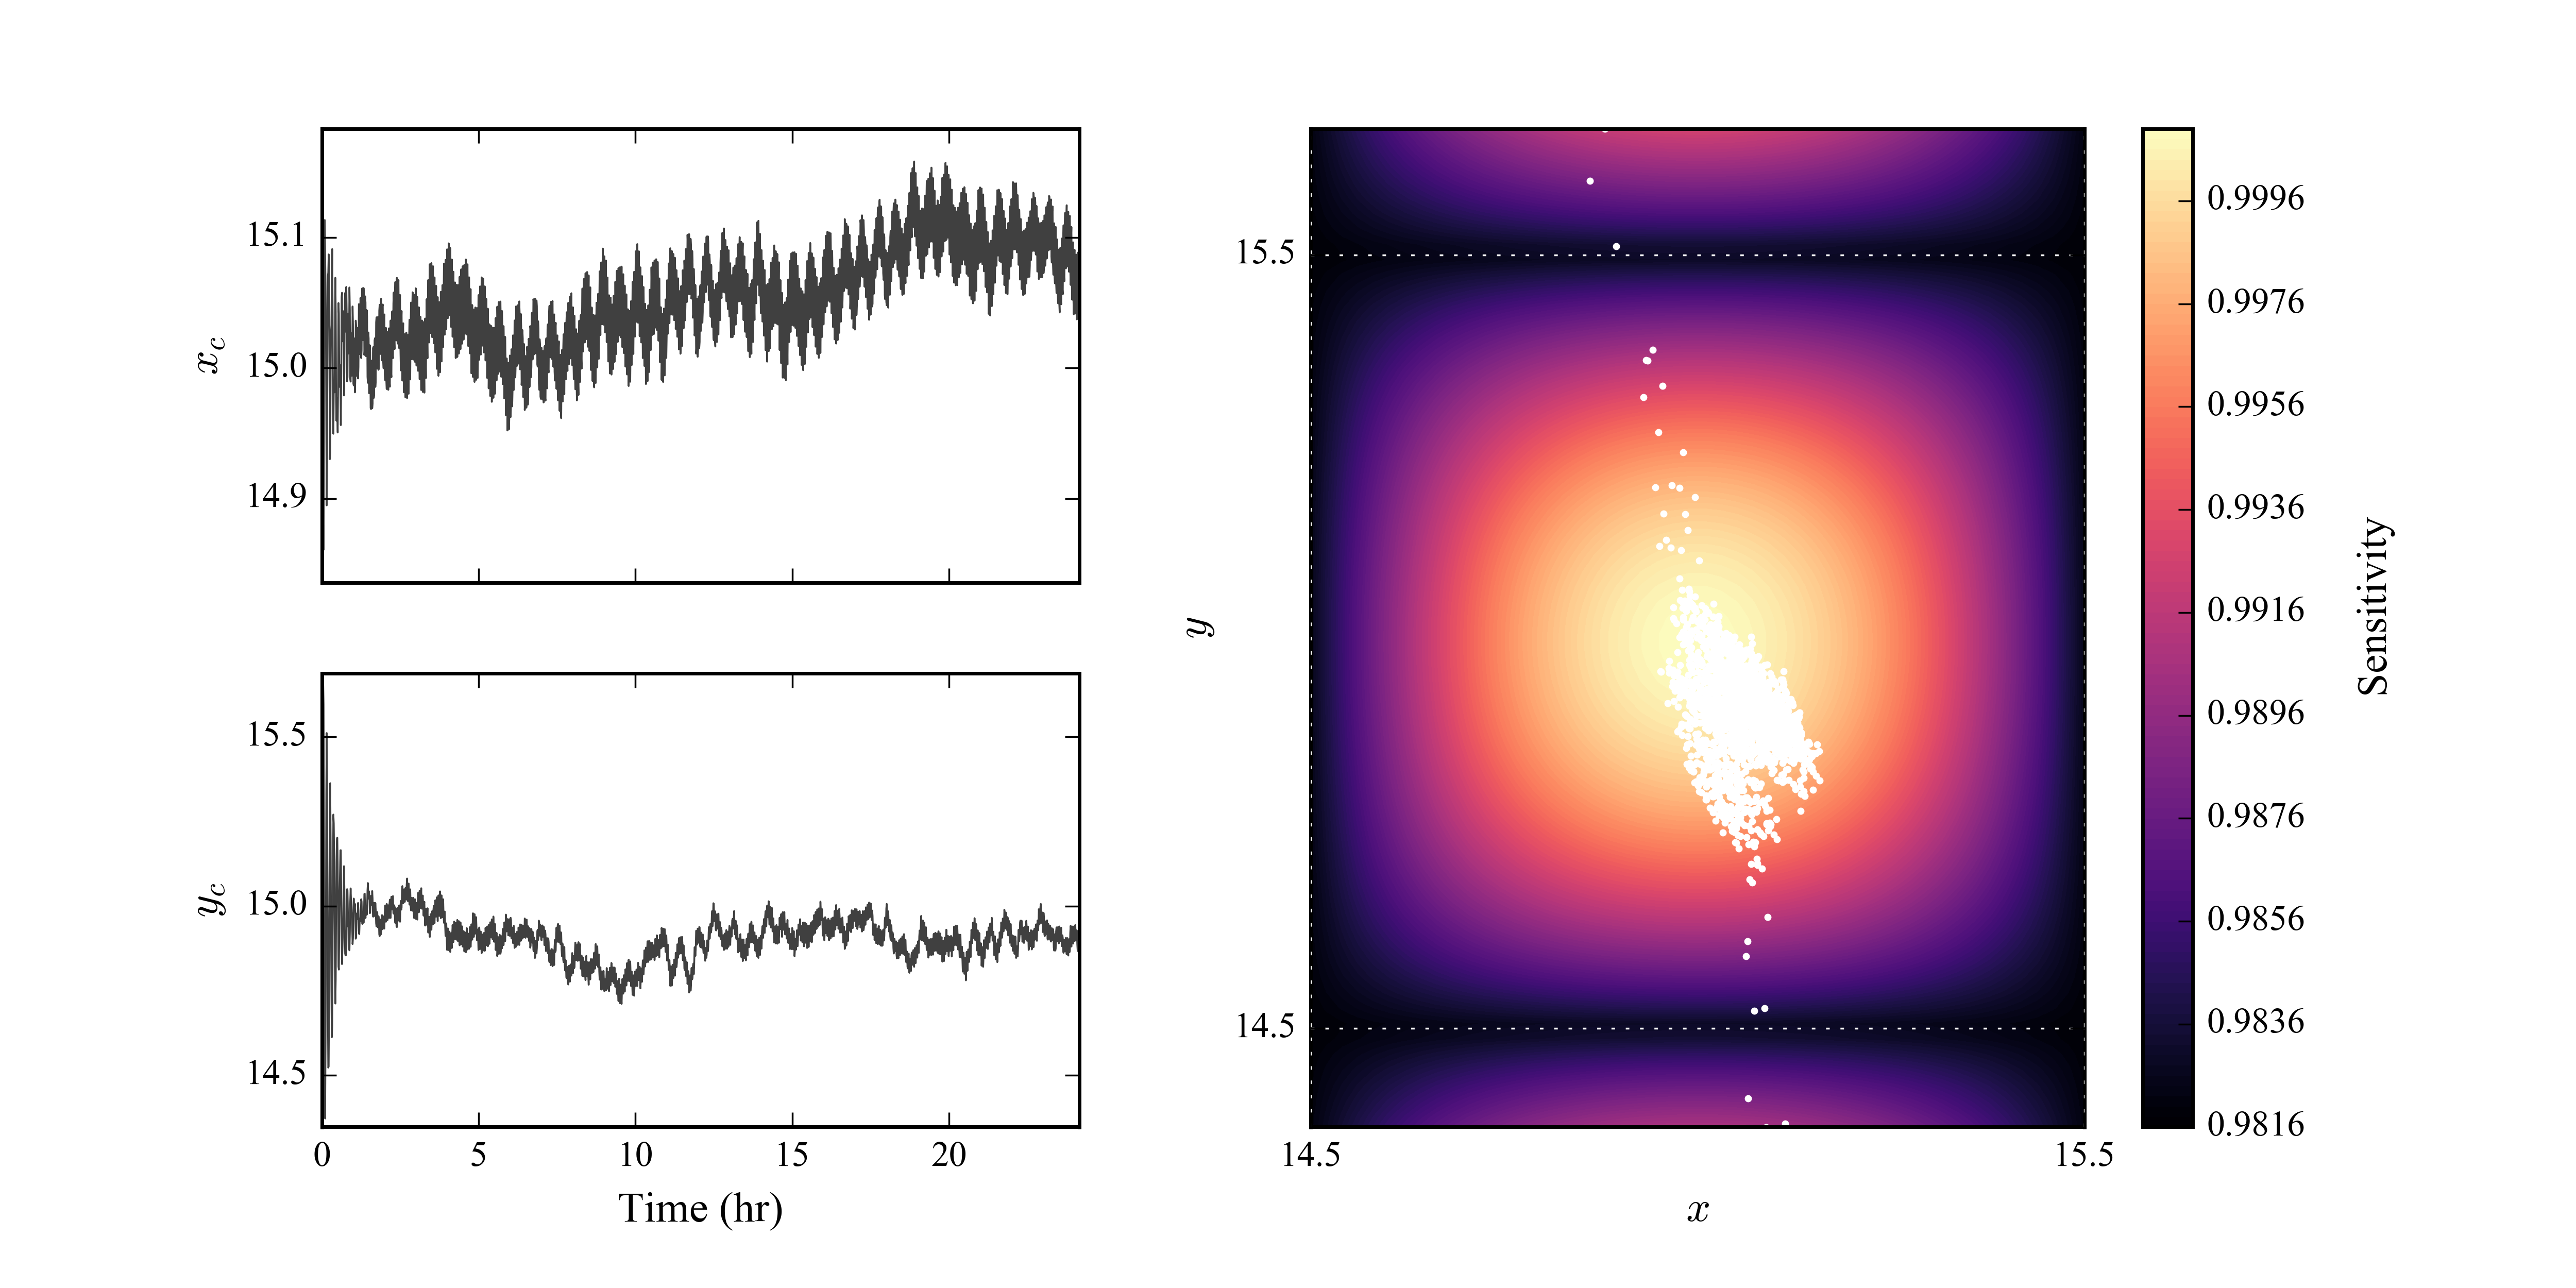
\includegraphics[width=\linewidth]{figs/smap_centroid.png}
 \caption{\small Synthetic IRAC data showing: (Left) Centroid position in $x$ and $y$ (in units of pixel side-length) with respect to time as determined by the center of light method. (Right) A map of intrapixel variability across three pixels (pixel boundaries are denoted by white). Sensitivity is in arbitrary units, normalized to the absolute flux of the star (no planet contribution). White points indicate samples of the centroid position over time. Synthetic data was generated using the method outlined in \citet{schwartz2016}. Data was simulated using the methods outlined in \citet{grillmair2014}.}
 \label{fig:sens_cent}
\end{figure*}

\begin{figure}

\subfloat{
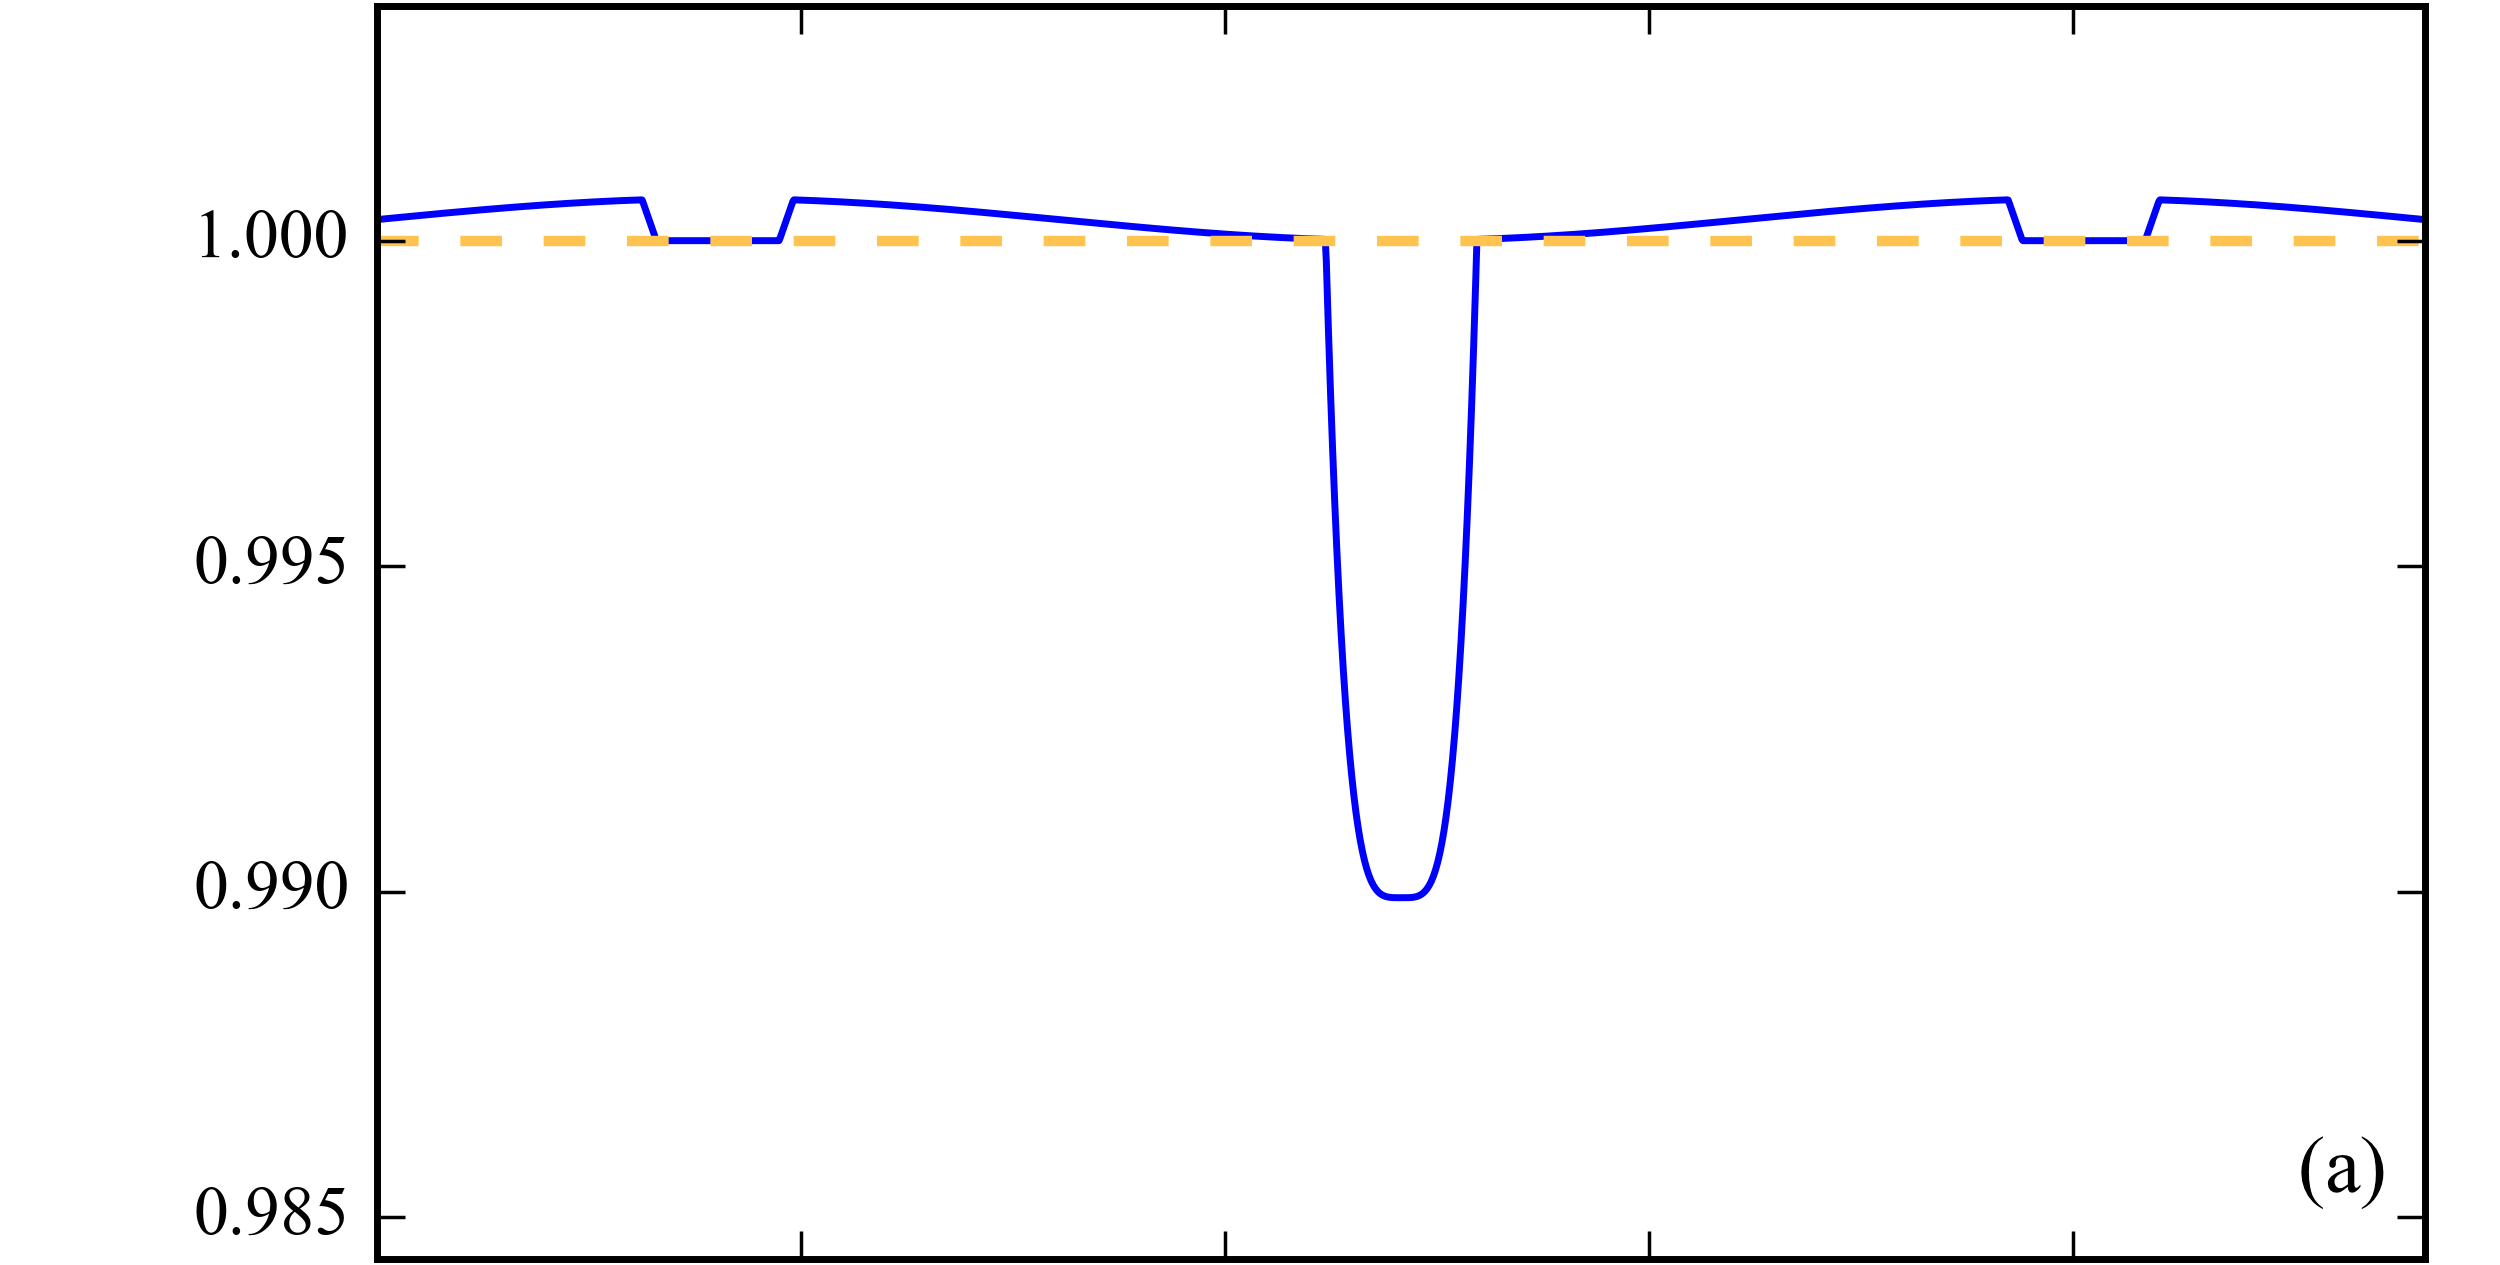
\includegraphics[clip,width=\columnwidth]{figs/stellar_flux.png}
\label{fig:astro}
}

\subfloat{
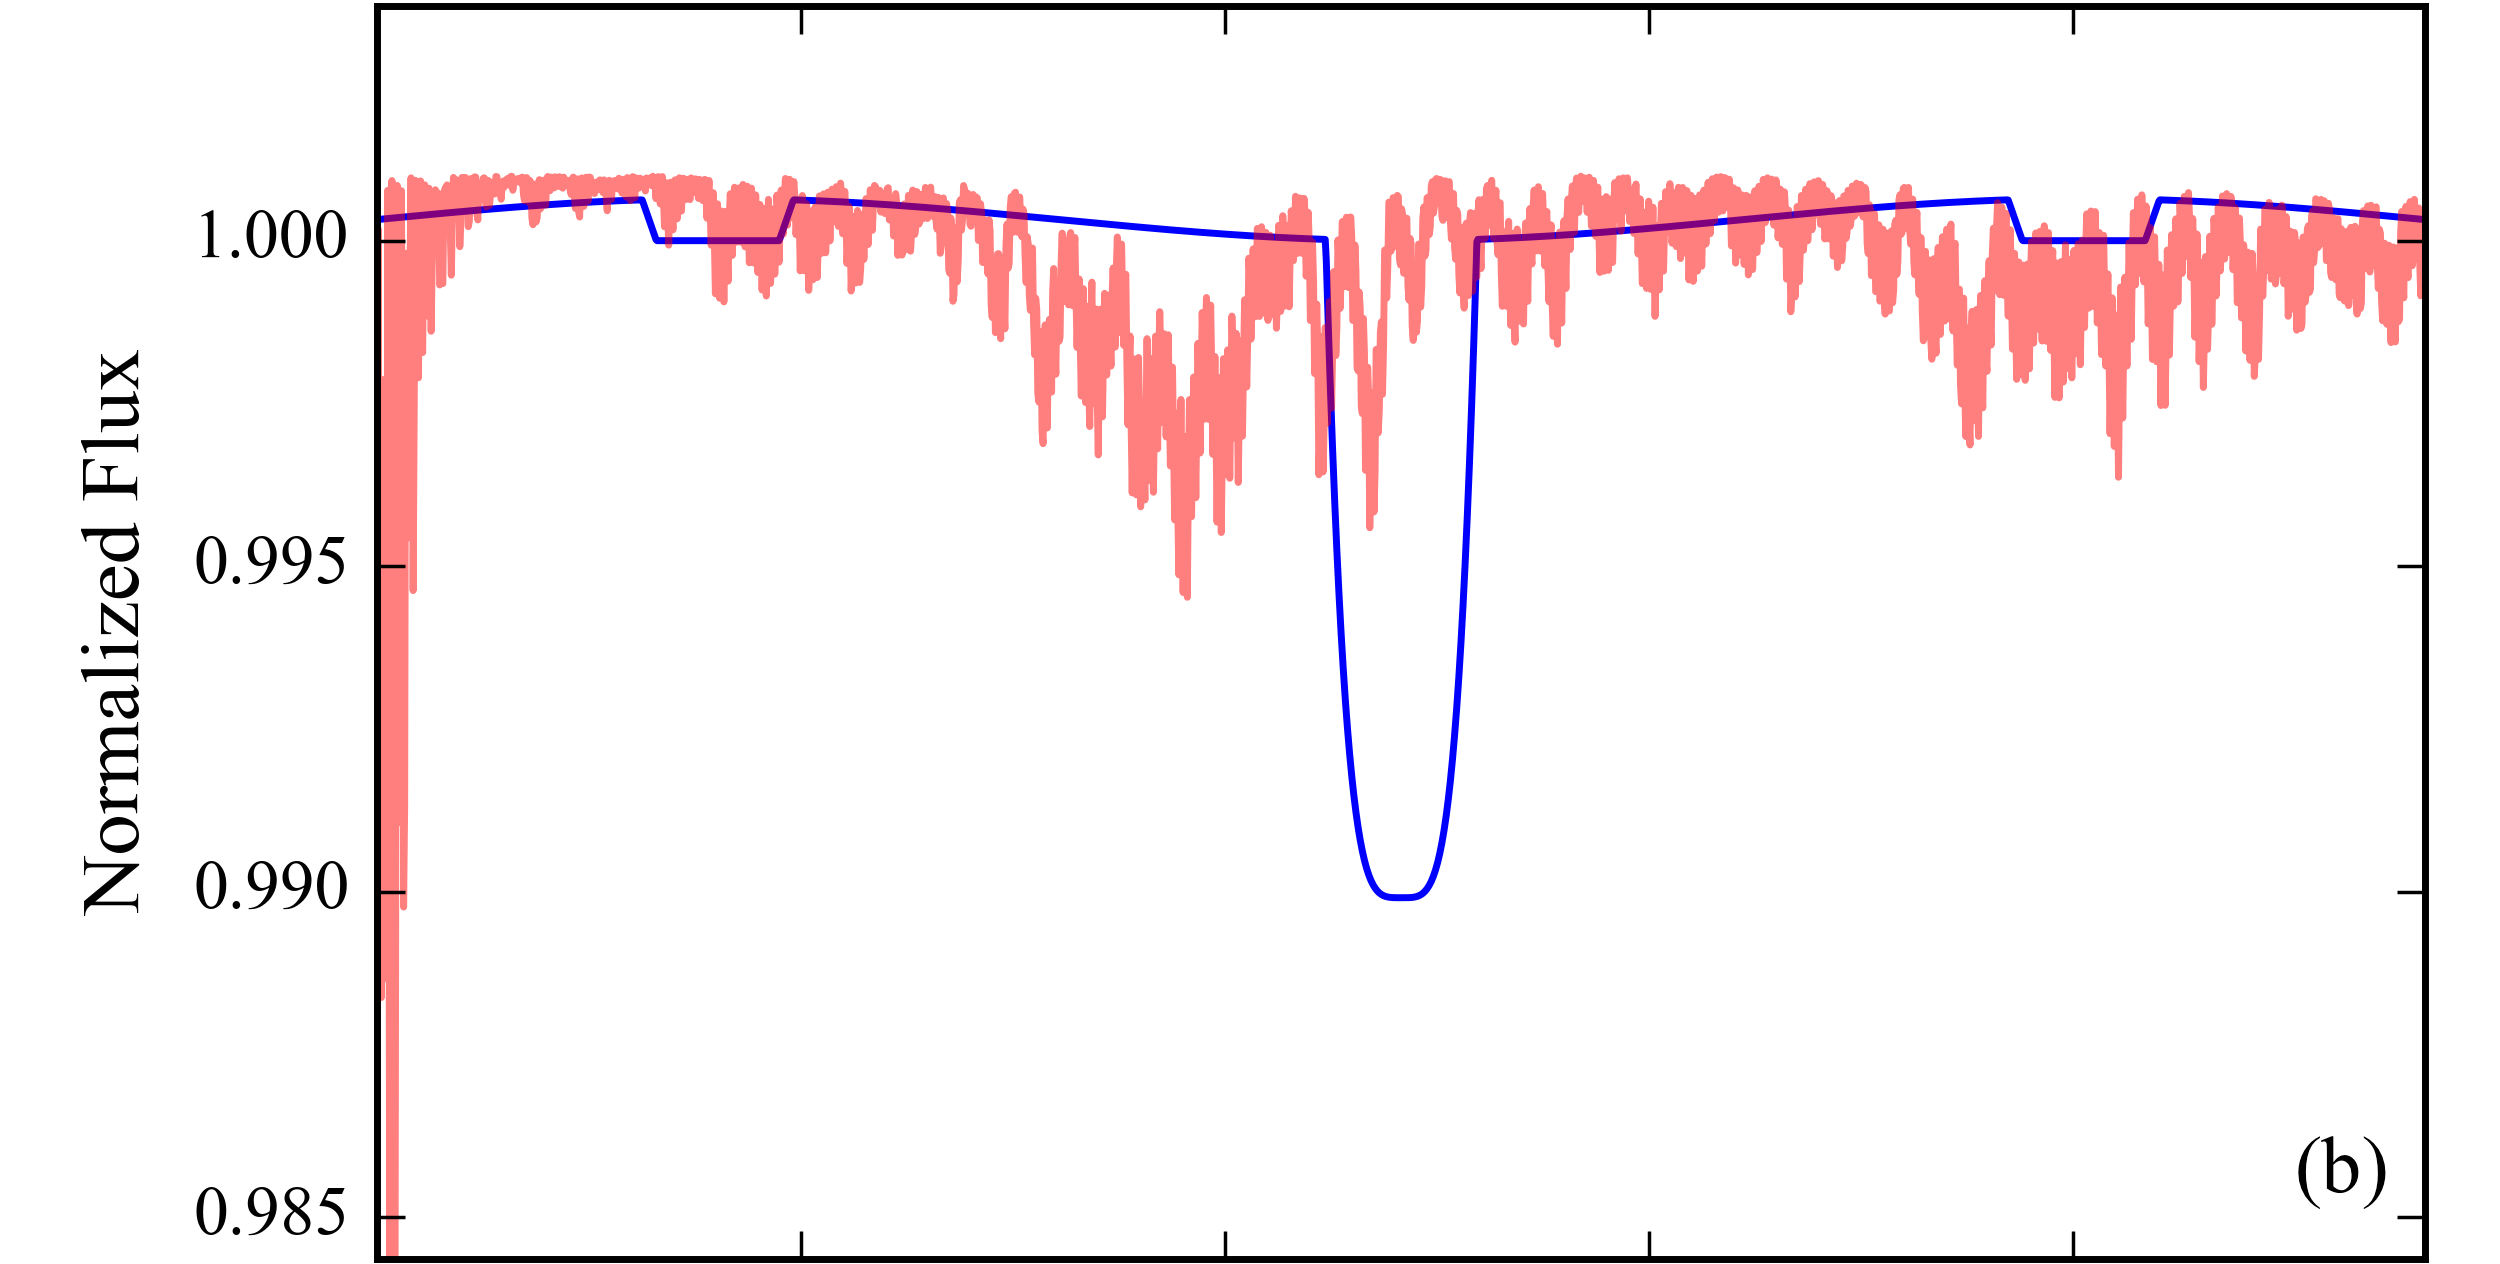
\includegraphics[clip,width=\columnwidth]{figs/stellar_detector.png}
\label{fig:detector}
}

\subfloat{
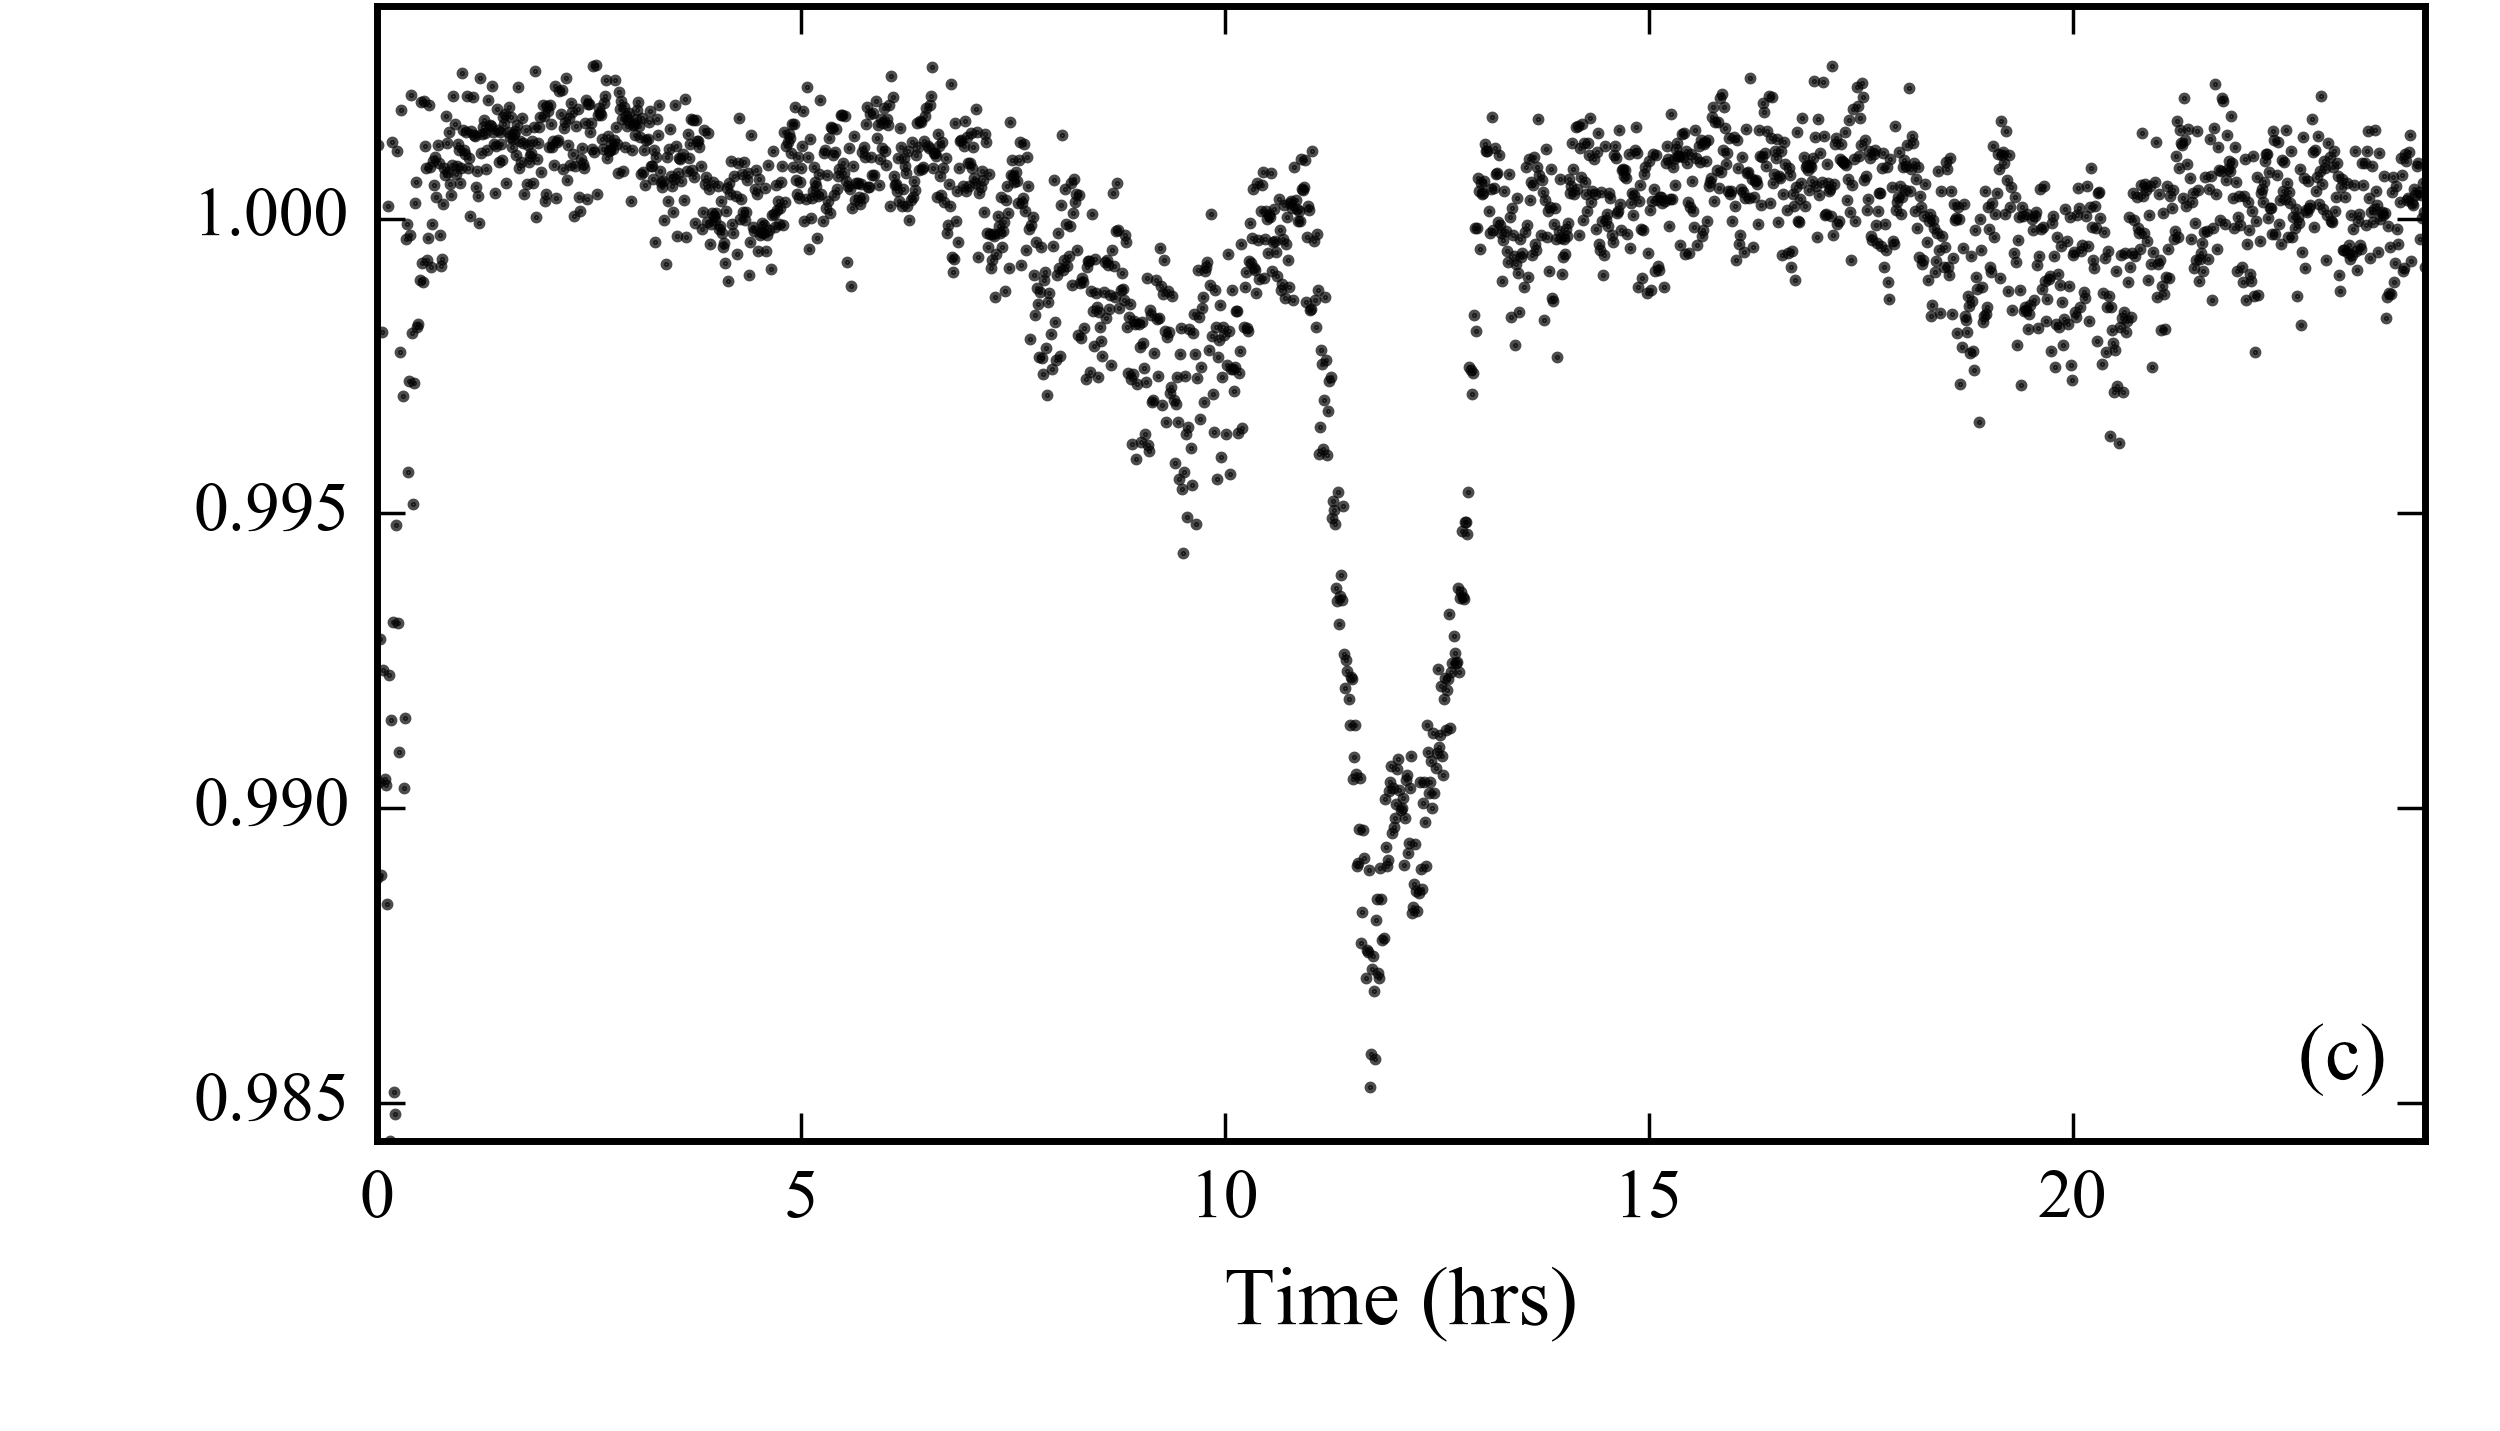
\includegraphics[clip,width=\columnwidth]{figs/stellar_data.png}
\label{fig:data}
}

\caption{\small (a): Yellow dashed line depicts the constant stellar flux (no exoplanet contribution). Blue line shows a plot of the astrophysical model outlined in \citet{schwartz2016}. (b): Red line depicts the synthetically generated detector model, as outlined in \citet{grillmair2014}, superimposed on the astrophysical model (blue line). (c): Data points draw from the product of the astrophysical and detector model, with each data point having additional Gaussian distributed noise (representative of the photon noise).}
\label{fig:synthetic_data}
\end{figure}

\section{Gaussian Processes}
\label{sec:gp}
Broadly, Gaussian process (GP) regression involves defining a likelihood function in terms of astrophysical and systematic parameters, and maximizing it with respect to the data. GP regression differs from other regression algorithms in that---in addition to allowing for variance on any single data point---covariance is allowed between data points. This results in off-diagonals in the covariance matrix. These covariant terms are not static, and are optimized to the data. They can be used to account for systematics whose functional form may not be understood from first principles. Here, parameters are split into two classes: astrophysical parameters, defining the physical planetary system, and hyperparameters, used to describe systematics. The likelihood function depends on the residuals between the astrophysical model and data, and the covariance matrix. The covariance matrix is calculated using a so-called kernel function.

\subsection{Kernel Functions}
\label{sec:kernel}
A kernel function is used to express similarity between data points. In our context, the purpose of the kernel function is to give a flexible description of the systematics. The choice of kernel for any given application therefore depends on the type of correlation expected in the data. Many classes of kernel function can be used, some of which are exotic and suited to very specific purposes (e.g. periodic kernels are implemented if periodic trends are expected in the covariance of the data).

A generic kernel is defined as
\begin{equation}
  k = k(\boldsymbol{v}_{i},\boldsymbol{v}_{j})\ ,
\end{equation}
where $\boldsymbol{v}_{i}$ and $\boldsymbol{v}_{j}$ are the $i^{th}$ and $j^{th}$ elements of the data input vector. In our analyses, $\boldsymbol{v}$ will be one of: the centroid position in $x$ or $y$, or the time ($x_{c}$, $y_{c}$ and $t$ respectively). For elements of $\boldsymbol{v}_{i}$ and $\boldsymbol{v}_{j}$ which are close in value, $k$ will return a value $\sim 1$, while for those that differ greatly in value, $k$ will return $\sim 0$.

The kernel used to characterize the $x$- and $y$-position on the pixel is the squared exponential kernel:
\begin{equation}
  k_{xy} = \omega_{xy}^{2} \, \mathrm{exp} \bigg[ - \, \Big(\, \frac{x_{i} - x_{j}}{L_x} \, \Big)^{2} - \,\Big(\,\frac{y_{i} - y_{j}}{L_y}\,\Big)^2\,\bigg],
\label{eq:kxy}
\end{equation}
where $x_{i}$ and $y_{i}$ are the centroid positions of the $i^{th}$ data point, $L_{x}$ and $L_{y}$ are the length scales over which intrapixel sensitivity variations are expected, and $\omega_{xy}$ is the weight associated with the kernel. This kernel indicates that, regardless of the functional form of the intrapixel variability, we expect similar regions of the pixel to exhibit similar sensitivity. Two points differing by several length scales, where systematics need not be related, would be assigned a covariance of $0$.

To model temporal variations, the $\frac{3}{2}$-Mat\'ern kernel was implemented, defined as:
\begin{equation}
  k_{t} = \omega_{t}^{2} \, \bigg(\sqrt{3}\,\frac{|t_{i} - t_{j}|}{L_t}\,\bigg)\,\mathrm{exp} \bigg[ - \, \Big(\, \sqrt{3}\,\frac{|t_{i} - t_{j}|}{L_t} \, \Big) \bigg]\ ,
\label{eq:kt}
\end{equation}
where $t_{i}$ is the corresponding time of the $i^{th}$ data point, $L_{t}$ is the timescale over which we expect the centroid to move significantly, and $\omega_{t}$ is the weight associated with the kernel.

The squared exponential kernel accounts for smooth variations in the data, while the Mat\'ern kernel accounts for residual correlated noise.

The effective kernel used in our analyses was the sum of these two kernels along with a term added to the diagonal, to account for Gaussian distributed noise in the data. This term effectively represents the variance of each data point due to photon noise, $\sigma^{2}$:
\begin{equation}
  k = k_{xy} + k_{t} + \sigma^{2}\ \delta_{i}^{j} ,
\end{equation}
where $\delta_{i}^{j}$ is the kronecker delta tensor. By applying the effective kernel to each combination of data points, a covariance matrix can be constructed as:
\begin{equation}
  [\mathrm{K}_{ij}] = k(\boldsymbol{v}_{i},\boldsymbol{v}_{j})
\label{eq:covmat}
\end{equation}

Figure \ref{fig:covmats} shows two example covariance matrices calculated with $k_{xy}$ and $k_{t}$ respectively, as well as the final effective covariance matrix. Note that the hyperparameters for this example were not optimized to the data set. The covariance matrix $\boldsymbol{\mathrm{K}}$ expresses all similarities in the data and is one of the main components of the GP likelihood function.

\begin{figure*}
  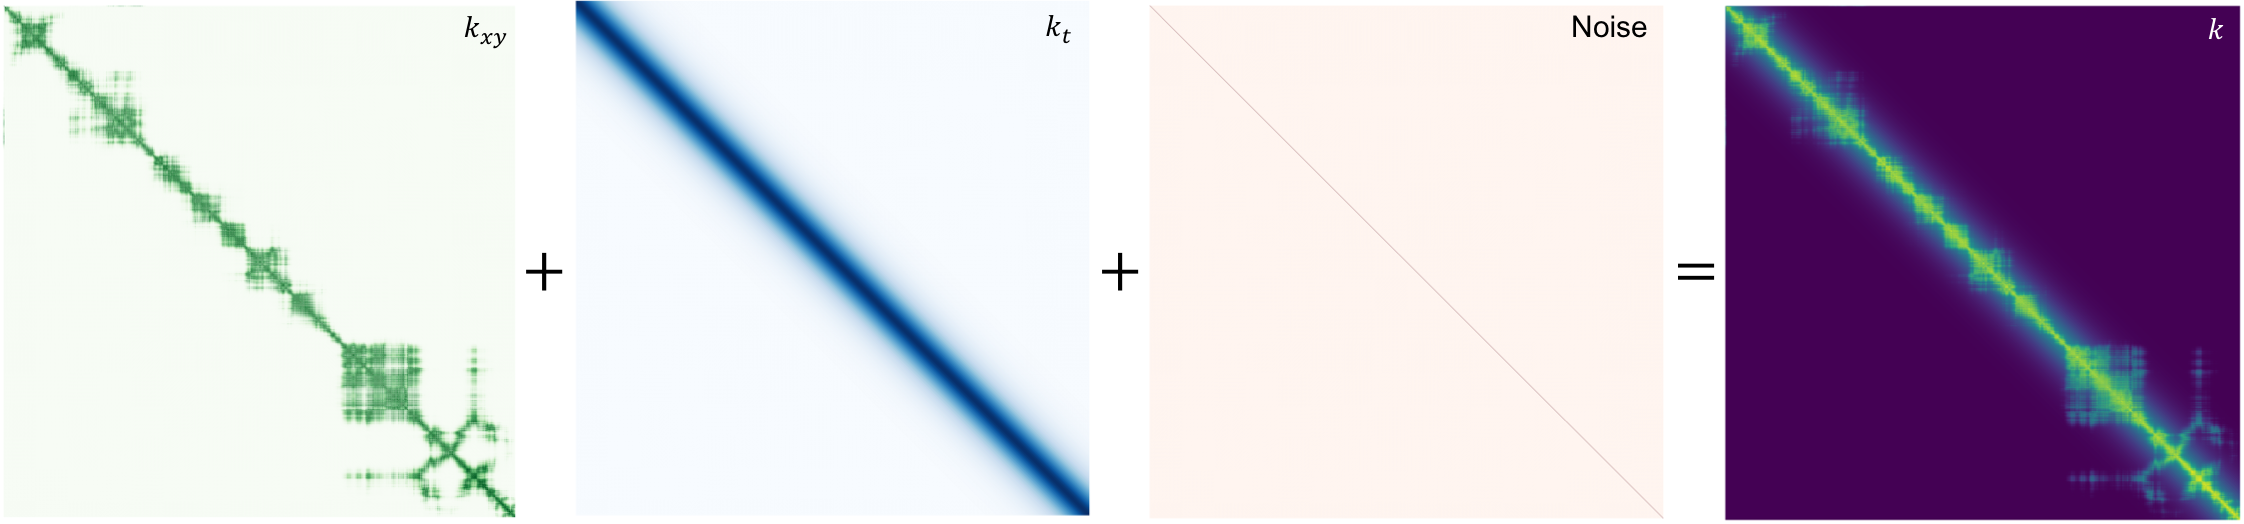
\includegraphics[width=\linewidth]{figs/covmats.png}
  \caption{\small From left to right: Plots of the squared exponential kernel ($k_{xy}$), the $\frac{3}{2}$-Mat\'ern kernel ($k_{t}$), Gaussian noise ($Noise$) and the sum of the three, ($k$). Colour saturation indicates high correlation. The final effective covariance matrix, $k$, should contain all information regarding pixel systematics.}
  \label{fig:covmats}
\end{figure*}

\subsection{The Likelihood Function}
\label{sec:lnp}
In a GP, every data point is associated with a normally distributed random variable \citep{rasmussen2006}. The probability to measure dataset $\boldsymbol{d} = (d_{1},...,d_{N})$ with standard deviation $\boldsymbol{\sigma} = (\sigma_{1},...,\sigma_{N})$, given an underlying astrophysical model $\boldsymbol{A} = (A_{1},...,A_{N})$ defined by parameters $\boldsymbol{\alpha}$ is
\begin{equation}
  \mathcal{P}(\boldsymbol{d}|\boldsymbol{\alpha}) =
   \prod_{i=1}^{N}\frac{1}{\sqrt{2\pi\sigma_{i}^{2}}}\, \mathrm{exp}\bigg[ - \, \frac{(d_{i} - A_{i})^{2}}{2\sigma_{i}^{2}}\, \bigg] = \mathcal{N}(\boldsymbol{A},\boldsymbol{\Sigma})\ ,
\label{eq:firstP}
\end{equation}
where $\mathcal{N}$ is a multivariate normal distribution and $\boldsymbol{\Sigma} = \mathrm{diag}[\boldsymbol{\sigma}]$ is the variance of the data, defined only along the diagonal. If we know modify this equation to include a covariance matrix with off-diagonals, as computed from equation \ref{eq:covmat}, we obtain the following likelihood
\begin{equation}
  \mathcal{P}(\boldsymbol{d}|\boldsymbol{\alpha},\boldsymbol{\gamma}) =  \mathcal{N}(\boldsymbol{A},\boldsymbol{\mathrm{K}}+\boldsymbol{\Sigma})\ ,
  \label{eq:P of KSig}
\end{equation}
where $\gamma = \{\omega_{xy},\omega_{t},L_{x},L_{y},L_{t}\}$ are the hyperparameters that define $\boldsymbol{\mathrm{K}}$. Computationally it is easiest to optimize the logarithm of this function. The loglikelihood function is then
\begin{equation}
  \mathrm{ln}\, \mathcal{P}(\boldsymbol{d}|\boldsymbol{\alpha},\boldsymbol{\gamma}) = -\frac{1}{2}\bigg[\boldsymbol{\mathrm{r}}^{\mathrm{T}}(\boldsymbol{\mathrm{K}} + \boldsymbol{\Sigma})^{-1}\boldsymbol{\mathrm{r}} + \mathrm{ln}\,|\boldsymbol{\mathrm{K}} \,+ \,\boldsymbol{\Sigma}| \,+\, N \mathrm{ln} \, (2\pi)\bigg]\ ,
  \label{eq:loglikeli}
\end{equation}
where $\boldsymbol{\mathrm{r}} = \boldsymbol{d} - \boldsymbol{A}$ is the residual vector between the data and the astrophysical model.

GP regression is effectively reduced to the optimization of Equation \ref{eq:loglikeli}. However, it may not be clear why this loglikelihood expression is a good framework to obtain estimates for $\boldsymbol{\alpha}$ and $\boldsymbol{\gamma}$. It is informative to break down the terms in equation \ref{eq:loglikeli} as
\begin{equation}
  \mathrm{ln}\, \mathcal{P}(\boldsymbol{d}|\boldsymbol{\alpha},\boldsymbol{\gamma}) = -\frac{1}{2}\bigg[ \chi ^{2} +Penalty + Const \bigg].
\end{equation}
The first term is a goodness-of-fit, similar to the $\chi ^{2}$. Its purpose is to minimize model residuals given the sensitivity of measurements encoded in $\boldsymbol{\mathrm{K}}$. This term is also the most computationally expensive and problematic process in a GP, as it involves inverting a large $N \times N$ matrix, where $N$ is the number of data points. This may become problematic when the matrix is sparse (as is often the case), and computationally scales on the order of $\mathcal{O}(N^{3})$. The second term penalizes model complexity. If the length scales $L_{x},L_{y},L_{t}$ become very small, this term decreases the likelihood, preventing overfitting. The GP regression therefore involves balancing the fit quality and model complexity. The final term is a normalization factor, which remains constant for a given dataset.

\subsection{Optimization}
\label{sec:optimization}
According to Bayes theorem, the probability that a given data set will result in the astrophysical parameters $\boldsymbol{\alpha}$ and hyperparameters $\boldsymbol{\gamma}$ is given by:
\begin{equation}
  \mathcal{P}(\boldsymbol{\alpha},\boldsymbol{\gamma}|\boldsymbol{d}) \propto \mathcal{P}(\boldsymbol{d}|\boldsymbol{\alpha},\boldsymbol{\gamma})\,\mathcal{P}(\boldsymbol{\alpha})\,\mathcal{P}(\boldsymbol{\gamma})\ ,
\end{equation}
where $\mathcal{P}(\boldsymbol{d}|\boldsymbol{\alpha},\boldsymbol{\gamma})$ is the loglikelihood from equation \ref{eq:loglikeli} and $\mathcal{P}(\boldsymbol{\alpha})$ and $\mathcal{P}(\boldsymbol{\gamma})$ are the respective prior probability distributions (priors) of the astrophysical and hyperparameters.

Uniform priors were chosen for all optimization variables. The bounds for the astrophysical parameters were applied liberally to be between $0$ and $10$ times the true value of the parameter, or in case of the phase offset within $\pm \pi / 2$, which encompasses all values accessible to the astrophysical model. The bounds for the hyperparameters were between $0$ and $2$ for the weights $\omega_i$, $0$ and $1$ for the spatial length scales $L_{x}$ and $L_{y}$, $0$ and the total observation time of a data set for the temporal length scale $L_{t}$, and $0$ and $1$ for the noise $\sigma$.

At the beginning of an optimization process, initial values for the astrophysical- and hyperparameters were drawn randomly from the priors. The drawn values were used to initialize a Nelder-Mead Simplex optimization algorithm---using the \texttt{Lmfit} python library--- to obtain maximum likelihood estimates (MLE) of Equation \ref{eq:loglikeli} \citep{neldermead1965, lmfit2014}. Since the covariance matrix had to be recomputed and inverted at each new iteration of hyperparameters, the optimization routine turned out to be computationally expensive and was prone to over- and underflow errors. An efficient and numerically stable computation was achieved  by applying a Cholesky decomposition, which exploits the positive-definite property of the covariance matrix and solves the inversion problem as a system of linear equations.

The Nelder-Mead optimization was repeated ten times, with different parameter initializations at each repetition. This was done to prevent optimizing to a local minimum of the likelihood surface. From the ten optimization routines, the parameters of the run which maximized the likelihood were chosen and used for further analysis.

In order to make the following sampling routines computationally tractable, the hyperparameters were kept fixed at their MLEs from this point onward. It should be noted however, that fixing the hyperparameters is not analogous to fixing the parameters of an explicit functional systematic model, but instead amounts to selecting a family of parametric models to characterize the high-level properties of the systematics \citep{evans2015}.

For additional exploration of the likelihood space as well as obtaining error estimates for the astrophysical parameters, an MCMC Ensemble Sampler was implemented using the python library \texttt{emcee} \citep{foreman2013,goodman2010}. 10 walkers per parameters were used for any given optimization routine. The walkers were initialized in a small locus around the MLEs of the parameters determined by the previous Nelder-Mead optimization. With these general guidelines in mind, the transit and eclipse parameters were then fit separately for a more efficient exploration of the parameter space. The resulting sample chains were then cleaned by truncating an initial period and slicing to eliminate autocorrelations.

\section{Results}

\begin{figure}[b]
  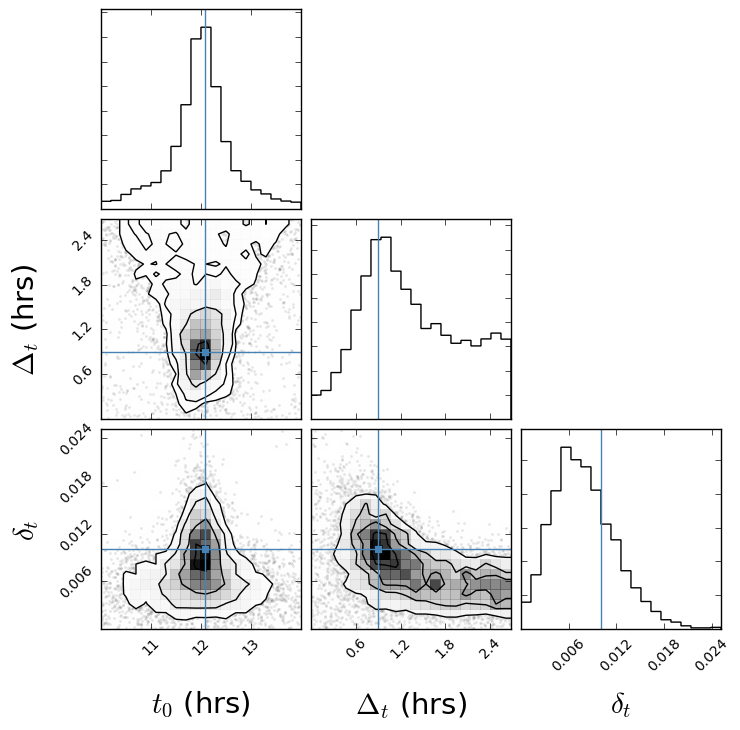
\includegraphics[width=0.8\linewidth]{figs/results/transit/transit_corner.png}
  \caption{\small The posterior distribution of the transit parameters from the MCMC chains. The contour plots indicate the density of samples of two given parameters while the histograms show the marginalized distribution for each individual parameter. $t_{c}$ is the transit center, $\Delta_{t}$ is the transit half-width and $\delta_{t}$ is the transit depth in units of normalized flux. The blue lines indicate the position of the true synthetic values.}
  \label{fig:transCorner}
\end{figure}

\begin{figure}[b]
  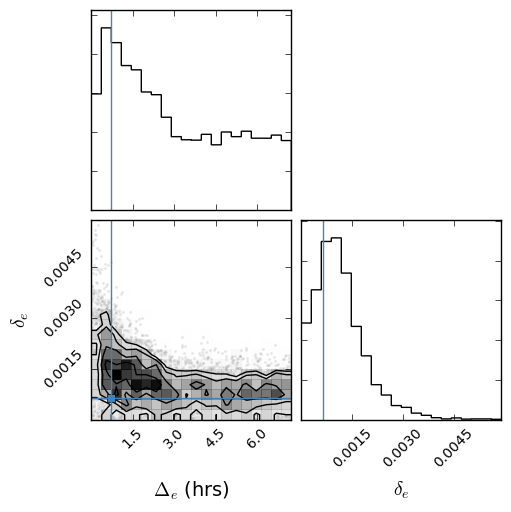
\includegraphics[width=\columnwidth]{figs/results/eclipse/eclipse_corner.png}
  \caption{\small The posterior distribution of the eclipse parameters from the MCMC chains. The contour plots indicate the density of samples of two given parameters while the histograms show the marginalized distribution for each individual parameter. $\Delta_{e}$ is the eclipse half-width and $\delta_{e}$ is the eclipse depth in units of normalized flux. The blue lines indicate the position of the true synthetic values.}
  \label{fig:eclCorner}
\end{figure}

\begin{figure}
  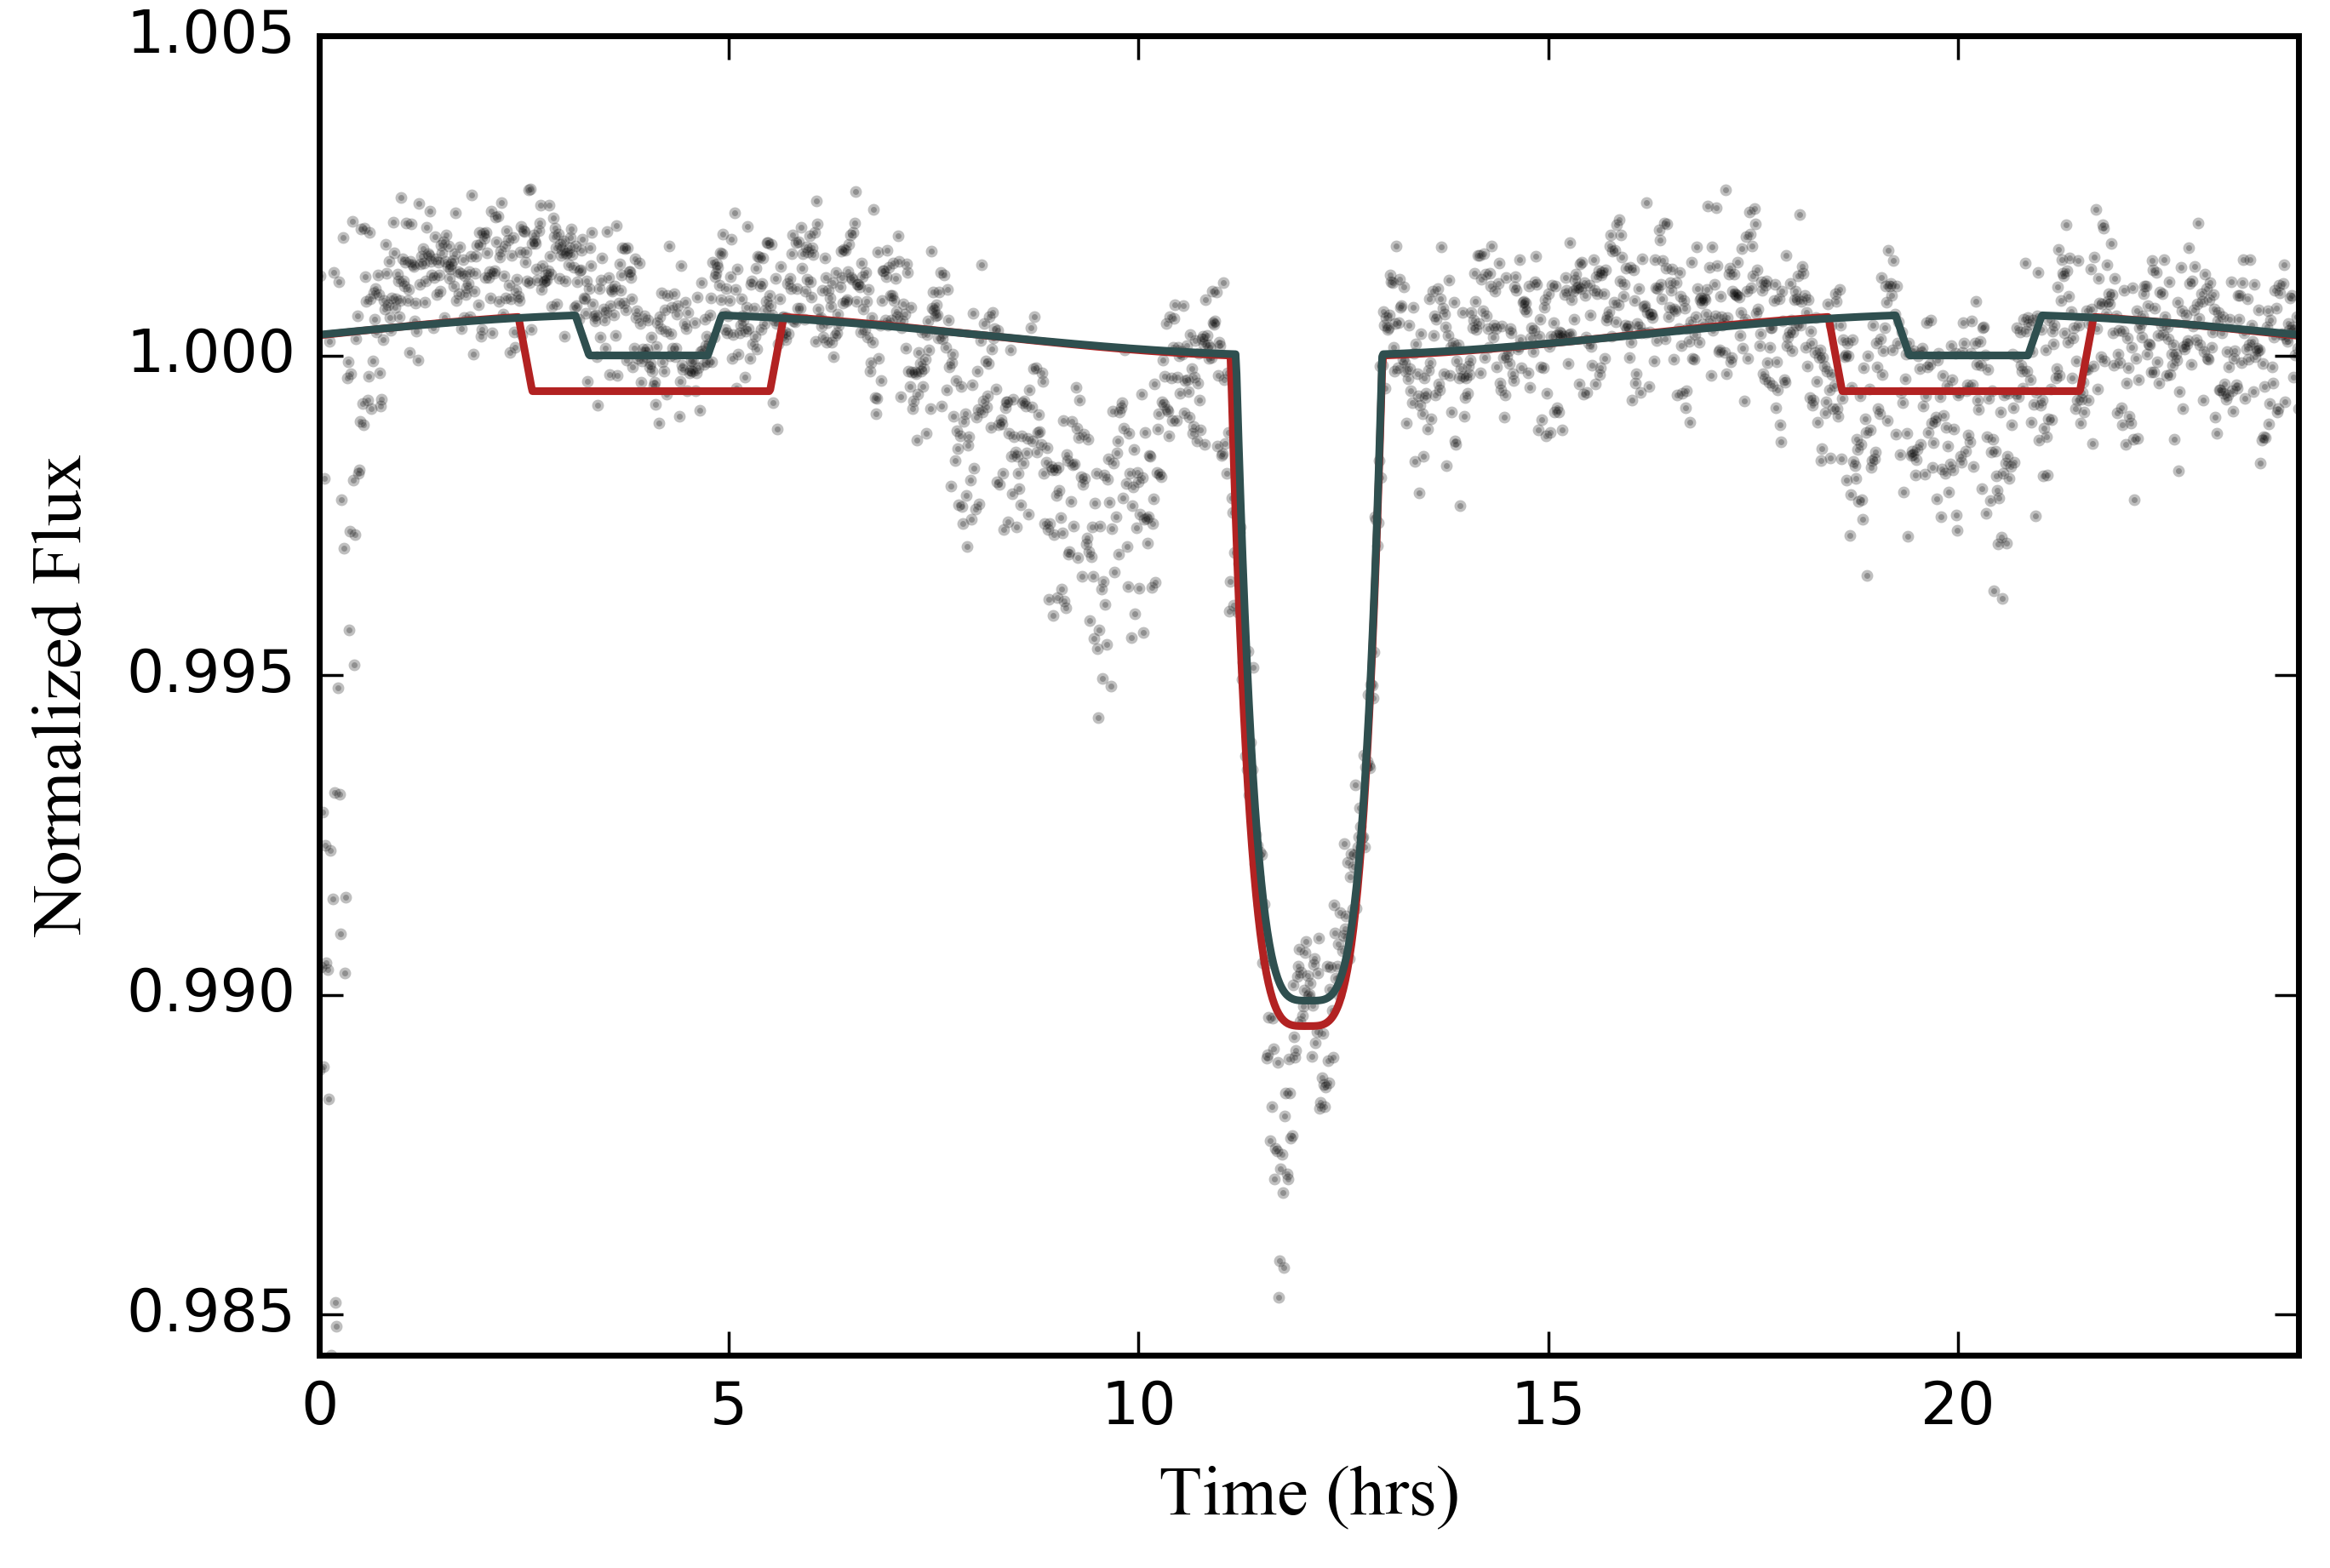
\includegraphics[width=\columnwidth]{figs/results/finalLC.png}
  \caption{Blue curve depicts the true synthetic astrophysical model. Black points show the full synthetic data, being a combination of the astrophysical model, detector model and photon noise. The red curve is our best fit model, using the parameters which maximized the loglikelihood function.}
  \label{fig:finalLC}
\end{figure}

\label{sec:results}
Regarding the transit, we ran an MCMC to sample the following parameters: the transit center, $t_c$, the transit half-width, $\Delta_{t}$, and the transit depth, $\delta_{t}$. The posterior distribution obtained from sampling the space of transit parameters is shown in Figure \ref{fig:transCorner}. We quote the median values, with errors ranging the central $68\%$ spread, in Table \ref{tbl:transitvalues}.

In regard to the secondary eclipse, the MCMC was sampled for the following parameters: the eclipse half-width, $\Delta_{e}$, and the eclipse depth, $\delta_{e}$. The posterior distribution obtained from sampling the space of eclipse parameters is shown in Figure \ref{fig:eclCorner}. We quote the median values, with errors ranging the central $68\%$ spread, in Table \ref{tbl:eclvalues}.

Due to the skew nature of the probability distribution, the MLEs do not coincide with the median probability parameters. As such, we have quoted the median values, with errors defined by the values encompassing $68\%$ of the data in Tables \ref{tbl:transitvalues} and \ref{tbl:eclvalues}. Alternatively, our best fit parameters are given by the MLEs, which have less reliable error estimates. The MLEs for the astrophysical and hyperparameters are shown in Table \ref{tbl:MLE}. The best fit curve is plotted in Figure \ref{fig:finalLC} along with the original light curve generated with the true values.

\section{Discussion}
\label{sec:discussion}
Figure \ref{fig:finalLC} shows our final best-fit astrophysical model, in comparison to the true synthetic model used to generate the data. The parameters describing the transit are closer to the genuine values than are the eclipse parameters. The can most likely be explained by how weak the eclipse signal is in comparison to the signal of the transit, potentially to such a degree that sensitivity variations and noise become dominant for the eclipse signal. We consider how the type of Gaussian process regression presented here can be applied to future experiments. 

IRAC's $5.8$ and $8.0~\mathrm{\mu m}$ channels implement silicon arsenic (Si:As) as the semi-conducting material \citep{evans2015}. An effect known as detector ramp has been observed in these detectors, in which the measured flux smoothly increases or decreases with time before reaching a steady-state value \citep{evans2015}. In the $8.0~\mathrm{\mu m}$ channel, this effect has been attributed to charge trapping, where photons saturate traps in the detector and thus increase the overall flux of electrons \citep{knutson2009}. It has been acknowledged, however, that theoretical models of these detectors are lacking, and systematics observed in the $5.8~\mathrm{\mu m}$ detector remain unexplained \citep{seager2010}.

In principle, the GP regression model outlined in this paper could be extended to model these detector ramp systematics. This could be done by including in the effective kernel an exponential squared kernel, dependent on some parameter describing the timescale of the ramp effect. This kernel should be able to encode the steep initial increase/decrease of sensitivity with respect to time, followed by the level-off \citep{evans2015}.

Modelling detector ramp effect would also be useful for the next generation of instruments. The James Webb Space Telescope (JWST) is a project led by the NASA with major contributions from the European and Canadian Space Agencies (ESA and CSA) \citep{gardner2006}. It is a space-based observatory, that will measure at infrared (IR) wavelengths ($\sim 0.6 - 28.5~\mathrm{\mu m}$) \citep{gardner2006}. As such, it will be of paramount use to exoplanet studies. The Mid-Infrared Instrument (MIRI) aboard the JWST will be the most well-suited instrument to study exoplanet transit photometry. Similar to \textit{Spitzer}/ IRAC's $5.8$ and $8.0~\mathrm{\mu m}$ channels, MIRI will be composed of Si:As detectors, arranged in an extended $1024\times 1024$ pixel format \citep{rieke2015}. We expect these detectors to exhibit similar detector ramp effects as those described above and thus a similar extension of our method could apply to data from this instrument.

\begin{table}[h!]
\centering
\caption{\small Results of the MCMC chains for the transit parameters. The values quoted are the median of each of the chains with ranges indicating the central $68\%$ spread of the samples around the median.}
\label{tbl:transitvalues}
\begin{tabular}{lll}
\multicolumn{1}{c}{$t_{0}$ (hrs)}      & \multicolumn{1}{c}{$\Delta_{t}$ (hrs)}     & \multicolumn{1}{c}{$\delta_{t}$} \\
\hline
\multicolumn{1}{c}{$12.01\,^{+0.49}_{-0.54}$} & \multicolumn{1}{c}{$1.23\,^{+0.94}_{-0.53}$} & \multicolumn{1}{c}{$(7.5\,^{+4.4}_{-3.4})\times 10^{-3}$}
\end{tabular}
\end{table}

\begin{table}[h!]
\centering
\caption{\small Results of the MCMC chains for the eclipse parameters. The values quoted are the median of each of the chains with ranges indicating the central $68\%$ spread of the samples around the median.}
\label{tbl:eclvalues}
\begin{tabular}{ll}
\multicolumn{1}{c}{$\Delta_{e}$ (hrs)}     & \multicolumn{1}{c}{$\delta_{e}$} \\
\hline
\multicolumn{1}{c}{$2.5\,^{+3.2}_{-1.7})$} & \multicolumn{1}{c}{$(1.03\,^{+0.78}_{-0.57})\times 10^{-3}$}
\end{tabular}
\end{table}

\begin{table*}[p]
\centering
\caption{Table of the MLEs for each parameter (hyper-, transit and eclipse). The true values of the astrophysical parameters are shown for comparison.}
\label{tbl:MLE}
\begin{tabular}{lccccccccccc}
      & $\omega_{xy}$ & $L_{x}$                & $L_{y}$                & $\omega_{t}$ & $L_{t}$ & $\sigma$ & $t_{0}$  & $\Delta_{t}$ & $\delta_{t}$ & $\Delta_{e}$ & $\delta_{e}$ \\
      & (\%)          & (pix)                  & (pix)                  & (\%)         & (mins)  & (ppm)    & (hrs)    & (hrs)        &     & (hrs)        &     \\ \cline{2-12}
MLE:  & $99.96$       & $1.078 \times 10^{-4}$ & $1.327 \times 10^{-3}$ & $13.98$      & $3.667$ & $2890$   & $12.050^{+0.47}_{-0.41}$ & $0.92$       & $1.046\times 10^{-2}$    & $1.45$       & $1.22 \times 10^{-3}$    \\
True: & ---           & ---                    & ---                    & ---          & ---     & ---      & $12.078$ & $0.89$       & $1.009\times 10^{-2}$    & $0.72$       & $0.65\times 10^{-3}$
\end{tabular}
\end{table*}

\section{Conclusion}
\label{sec:conclusion}
In this paper, we have presented an analysis of synthetic \textit{Spitzer}/ IRAC exoplanet light curves using Gaussian Process regression. The median values for transit center, half-width, and relative depth were found to be $(12.01\,^{+0.49}_{-0.54})\ \mathrm{hrs}$, $(1.23\,^{+0.94}_{-0.53})\ \mathrm{hrs}$, $(7.5\,^{+4.4}_{-3.4})\times 10^{-3}$ respectively, in agreement with the true values of $(12.078)\ \mathrm{hrs}$, $(0.89)\ \mathrm{hrs}$ and $10.46\times 10^{-3}$. The median values for eclipse half-width and relative depth were found to be $(2.5\,^{+3.2}_{-1.7})\ \mathrm{hrs}$ and $(1.03\,^{+0.78}_{-0.57})\times 10^{-3}$, in agreement with the true values of $(0.72)\ \mathrm{hrs}$ and $0.65\times 10^{-3}$. We conclude that Gaussian process regression offers a viable alternative for IRAC light curve fitting.
\pagebreak
\section{Acknowledgements}
We would like to express our sincere gratitude to our advisors Dr. Joel C. Schwartz and Professor Nicolas B. Cowan for their continued support and guidance over the course of this project, the Cowan group for putting up with our bad jokes during group meetings and of course, our idols, William Rasmussen, Daniel Foreman-Mackey and Thomas Evans.

%% The reference list follows the main body and any appendices.
%% Use LaTeX's thebibliography environment to mark up your reference list.
%% Note \begin{thebibliography} is followed by an empty set of
%% curly braces.  If you forget this, LaTeX will generate the error
%% "Perhaps a missing \item?".
%%
%% thebibliography produces citations in the text using \bibitem-\cite
%% cross-referencing. Each reference is preceded by a
%% \bibitem command that defines in curly braces the KEY that corresponds
%% to the KEY in the \cite commands (see the first section above).
%% Make sure that you provide a unique KEY for every \bibitem or else the
%% paper will not LaTeX. The square brackets should contain
%% the citation text that LaTeX will insert in
%% place of the \cite commands.

%% We have used macros to produce journal name abbreviations.
%% \aastex provides a number of these for the more frequently-cited journals.
%% See the Author Guide for a list of them.

%% Note that the style of the \bibitem labels (in []) is slightly
%% different from previous examples.  The natbib system solves a host
%% of citation expression problems, but it is necessary to clearly
%% delimit the year from the author name used in the citation.
%% See the natbib documentation for more details and options.

\begin{thebibliography}{38}
\providecommand{\natexlab}[1]{#1}
\providecommand{\url}[1]{\texttt{#1}}
\expandafter\ifx\csname urlstyle\endcsname\relax
  \providecommand{\doi}[1]{doi: #1}\else
  \providecommand{\doi}{doi: \begingroup \urlstyle{rm}\Url}\fi

\bibitem[Agol et al.(2010)]{agol2010} Agol, E., Cowan, N.~B., Knutson, H.~A., et al.\ 2010, \apj, 721, 1861

\bibitem[Ballard et al.(2010)]{ballard2010} Ballard, S., Charbonneau, D., Deming, D., et al.\ 2010, \pasp, 122, 1341

\bibitem[Carroll \& Ostlie(2006)]{carroll2006} Carroll, B.~W., \& Ostlie, D.~A.\ 2006, Institute for Mathematics and Its Applications,

\bibitem[Charbonneau et al.(2005)]{charbonneau2005} Charbonneau, D., Allen, L.~E., Megeath, S.~T., et al.\ 2005, \apj, 626, 523

\bibitem[Crossfield et al.(2012)]{crossfield2012} Crossfield, I.~J.~M., Knutson, H., Fortney, J., et al.\ 2012, \apj, 752, 81

\bibitem[Deming et al.(2006)]{deming2006} Deming, D., Harrington, J., Seager, S., \& Richardson, L.~J.\ 2006, \apj, 644, 560

\bibitem[D{\'e}sert et al.(2009)]{desert2009} D{\'e}sert, J.-M., Lecavelier des Etangs, A., H{\'e}brard, G., et al.\ 2009, \apj, 699, 478

\bibitem[Evans et al.(2013)]{evans2013} Evans, T.~M., Pont, F., Sing, D.~K., et al.\ 2013, \apjl, 772, L16

\bibitem[Evans et al.(2015)]{evans2015} Evans, T.~M., Aigrain, S., Gibson, N., et al.\ 2015, \mnras, 451, 680

\bibitem[Fazio et al.(2004)]{fazio2004} Fazio, G.~G., Hora, J.~L., Allen, L.~E., et al.\ 2004, \apjs, 154, 10

\bibitem[Foreman-Mackey et al.(2013)]{foreman2013} Foreman-Mackey D., Hogg D.~W., Lang D., Goodman J.,\ 2013, \pasp, 125, 306

\bibitem[Gardner et al.(2006)]{gardner2006} Gardner, J.~P., Mather, J.~C., Clampin, M., et al.\ 2006, \ssr, 123, 485

\bibitem[Gibson et al.(2012{\natexlab{a}})]{gibson2012a} Gibson, N.~P., Aigrain, S., Pont, F., et al.\ 2012, \mnras, 422, 753

\bibitem[Gibson et al.(2012{\natexlab{b}})]{gibson2012b} Gibson, N.~P., Aigrain, S., Roberts, S., et al.\ 2012, \mnras, 419, 2683

\bibitem[Gibson et al.(2013{\natexlab{a}})]{gibson2013a} Gibson, N.~P., Aigrain, S., Barstow, J.~K., et al.\ 2013, \mnras, 428, 3680

\bibitem[Gibson et al.(2013{\natexlab{b}})]{gibson2013b} Gibson, N.~P., Aigrain, S., Barstow, J.~K., et al.\ 2013, \mnras, 436, 2974

\bibitem[Gibson(2014)]{gibson2014} Gibson, N.~P.\ 2014, \mnras, 445, 3401

\bibitem[Goodman \& Weare(2010)]{goodman2010} Goodman, J. \& Weare, J.\ 2010, Comm. App. Math. Comp. Sci., 5, 65

\bibitem[Grillmair et al.(2014)]{grillmair2014} Grillmair, C.~J., Carey, S.~J., Stauffer, J.~R., \& Ingalls, J.~G.\ 2014, \procspie, 9143, 914359

\bibitem[Ingalls et al.(2016)]{ingalls2016} Ingalls, J.~G., Krick, J.~E., Carey, S.~J., et al.\ 2016, \aj, 152, 44

\bibitem[Knutson et al.(2007)]{knutson2007} Knutson, H.~A., Charbonneau, D., Allen, L.~E., et al.\ 2007, \nat, 447, 183

\bibitem[Knutson et al.(2008)]{knutson2008} Knutson, H.~A., Charbonneau, D., Allen, L.~E., Burrows, A., \& Megeath, S.~T.\ 2008, \apj, 673, 526-531

\bibitem[Knutson et al.(2009)]{knutson2009} Knutson, H.~A., Charbonneau, D., Cowan, N.~B., et al.\ 2009, \apj, 703, 769

\bibitem[Knutson et al.(2012)]{knutson2012} Knutson, H.~A., Lewis, N., Fortney, J.~J., et al.\ 2012, \apj, 754, 22

\bibitem[Krick et al.(2016)]{krick2016} Krick, J.~E., Ingalls, J., Carey, S., et al.\ 2016, \apj, 824, 27

\bibitem[Lewis et al.(2013)]{lewis2013} Lewis, N.~K., Knutson, H.~A., Showman, A.~P., et al.\ 2013, \apj, 766, 95

\bibitem[Mayor \& Queloz(1995)]{mayor1995} Mayor, M., \& Queloz, D.\ 1995, \nat, 378, 355

\bibitem[Nelder \& Mead(1965)]{neldermead1965} Nelder, J. A. \& Mead, R.\ 1965, Computer Journal, 7, 308

\bibitem[Newville et al.(2014)]{lmfit2014} Newville M., Stensitzki T., Allen D., Ingargiola A.,\ 2014, Zenodo

\bibitem[Rasmussen \& Williams (2006)]{rasmussen2006} Rasmussen, C.~E., Williams, C.~K.~I.\ 2006, Gaussian Processes for Machine Learning (Cambridge, Massachusetts, USA: MIT Press)

\bibitem[Reach et al.(2005)]{reach2005} Reach, W.~T., Megeath, S.~T., Cohen, M., et al.\ 2005, \pasp, 117, 978

\bibitem[Rieke et al.(2015)]{rieke2015} Rieke, G.~H., Ressler, M.~E., Morrison, J.~E., et al.\ 2015, \pasp, 127, 665

\bibitem[Schwartz \& Cowan(2016)]{schwartz2016} Schwartz, J.~C., \& Cowan, N.~B.\ 2016, arXiv:1607.01013

\bibitem[Seager \& Deming(2010)]{seager2010} Seager, S., \& Deming, D.\ 2010, \araa, 48, 631

\bibitem[Stevenson et al.(2012)]{stevenson2012} Stevenson, K.~B., Harrington, J., Fortney, J.~J., et al.\ 2012, \apj, 754, 136

\bibitem[Todorov et al.(2014)]{todorov2014} Todorov, K.~O., Deming, D., Burrows, A., \& Grillmair, C.~J.\ 2014, \apj, 796, 100

\bibitem[van den Bos(1943)]{vandenbos1943} van den Bos, W.~H.\ 1943, Monthly Notes of the Astronomical Society of South Africa, 2, 14

\bibitem[Werner(2009)]{werner2009} Werner, M.\ 2009, American Scientist, 97, 458

\end{thebibliography}

\end{document}

% End of file `hoffart-lamberti-459-final.tex'.
